\documentclass[
oneside,							% einseitiges Layout
captions=signature,	  % caps immer unter Element (Bild, Grafik...)
openany,							% Kapitel können auch auf linken Seiten beginnen
listof=totoc				% Abb.- und Tab.verzeichnis im Inhalt	
]
{scrbook}


\usepackage[utf8]{inputenc}
\usepackage[T1]{fontenc}

\usepackage{mathptmx}
\usepackage[scaled=.90]{helvet}
\usepackage{courier}
					
\usepackage[ngerman]{babel}

\usepackage{tikz}
\usepackage{qtree} % Baumstrukturen zeichnen

\usepackage{tabularx}
\usepackage{tabulary}
\usepackage{multirow}
\usepackage{colortbl}
\usepackage{booktabs}
\usepackage{listings}
\usepackage{verbatim}
\usepackage{textcomp}

\lstset{
  frame=l,
  basicstyle=\small\ttfamily,
  numbers=left,
  numberstyle=\tiny\color{gray},
  keywordstyle=\color{blue},
  commentstyle=\color{green}\ttfamily,
  stringstyle=\color{mauve},
  texcl=false,
	breaklines=true
}
\lstset{literate=
  {á}{{\'a}}1 {é}{{\'e}}1 {í}{{\'i}}1 {ó}{{\'o}}1 {ú}{{\'u}}1
  {Á}{{\'A}}1 {É}{{\'E}}1 {Í}{{\'I}}1 {Ó}{{\'O}}1 {Ú}{{\'U}}1
  {à}{{\`a}}1 {è}{{\`e}}1 {ì}{{\`i}}1 {ò}{{\`o}}1 {ù}{{\`u}}1
  {À}{{\`A}}1 {È}{{\'E}}1 {Ì}{{\`I}}1 {Ò}{{\`O}}1 {Ù}{{\`U}}1
  {ä}{{\"a}}1 {ë}{{\"e}}1 {ï}{{\"i}}1 {ö}{{\"o}}1 {ü}{{\"u}}1
  {Ä}{{\"A}}1 {Ë}{{\"E}}1 {Ï}{{\"I}}1 {Ö}{{\"O}}1 {Ü}{{\"U}}1
  {â}{{\^a}}1 {ê}{{\^e}}1 {î}{{\^i}}1 {ô}{{\^o}}1 {û}{{\^u}}1
  {Â}{{\^A}}1 {Ê}{{\^E}}1 {Î}{{\^I}}1 {Ô}{{\^O}}1 {Û}{{\^U}}1
  {Ã}{{\~A}}1 {ã}{{\~a}}1 {Õ}{{\~O}}1 {õ}{{\~o}}1
  {œ}{{\oe}}1 {Œ}{{\OE}}1 {æ}{{\ae}}1 {Æ}{{\AE}}1 {ß}{{\ss}}1
  {ű}{{\H{u}}}1 {Ű}{{\H{U}}}1 {ő}{{\H{o}}}1 {Ő}{{\H{O}}}1
  {ç}{{\c c}}1 {Ç}{{\c C}}1 {ø}{{\o}}1 {å}{{\r a}}1 {Å}{{\r A}}1
  {€}{{\euro}}1 {£}{{\pounds}}1 {«}{{\guillemotleft}}1
  {»}{{\guillemotright}}1 {ñ}{{\~n}}1 {Ñ}{{\~N}}1 {¿}{{?`}}1
}

%% Packages für Grafiken & Abbildungen %%%%%%%%%%%%%%%%%%%%%%

\usepackage{graphicx} 	% Zum Laden von Grafiken
\usepackage{xcolor}
\usepackage{color}
\usepackage{microtype} 	% visual enhancement randausgleich
\usepackage{float} 			% ermöglicht den H param bei Bilder 
					
					
												% für Plazierungen an der Position

\usepackage{rotating} % Text drehen
\usepackage{url}
\usepackage[nogroupskip, nonumberlist, toc]{glossaries}
\usepackage{glossary-inline}
\usepackage[printonlyused]{acronym}

\usepackage{pifont} 	%symbol fonts like Windings
\usepackage{amsmath}	% Math font optimisation
\usepackage{amssymb} 	% Math symbols

\usepackage{tocloft} % Table of content - list of figures, tables - management


%% Bibliographiestil %%%%%%%%%%%%%%%%%%%%%%%%%%%%%%%%%%%%%%%%%%%%%%%%%%

\usepackage{natbib}
\renewcommand{\familydefault}{\sfdefault}


\setlength{\parindent}{0cm}			% Absatzeinzug
\setlength{\parskip}{6pt}				% Leerzeile zwischen Absätzen im Inhaltsverzeichnis
\textwidth=15.7cm								% Textbreite
\leftmargin=-3cm

\textheight=22.6cm							% Texthöhe
\topmargin=-0.7cm								% Rand (Vorsicht minus)
\headheight=0.2cm								% Höhe der Kopfzeile
\headsep=1.5cm									% Abstand von der Kopfzeile zum Text

%\setlength{\bibsep}{0.4\parskip}   	 	%Bibliographieabstand fest
\setlength{\bibsep}{0.3em plus 0.5em}	
%Bibliographieabstand variabel um Seitenumbruch zu unterdrücken

\setlength{\bibhang}{1cm}    			%Bibliographieeinzug
%\newcommand{\bibfont}{\normalsize}   	%Bibliographiezeichengröße
\renewenvironment{quote}{\list{}{\rightmargin0pt\leftmargin1cm}\item\relax}{\endlist} 
% neue \quote-Definition als globale Variabel für rechtsbündige Zitate

\setcitestyle{notesep={: }}
\setcitestyle{aysep={}}

%%%%%%%%%%%%%%%%%%%%%%%%%%%%%%%\setlist{\setlength{\itemsep}{0.8em plus 2em}, parsep=.65em, partopsep=1em} %listenformatierung

%%%%%% TOC Tiefe %%%%%%%%%%%%%%%%%%%%%%%%%%%%%%%%%%%%%
\setcounter{tocdepth}{3}

%%%%%%%% Nummerierungstiefe absätze %%%%%%%%%%%%%%%%%%
\setcounter{secnumdepth}{3}

%\setkomafont{section}{\LARGE}
%\setkomafont{subsection}{\Large}
%\setkomafont{subsubsection}{\large}
%\setkomafont{paragraph}{\large}
%\setkomafont{subparagraph}{\large}
% Die Überschriften sind in der Lokalen *.cls 
% Classendefinition definiert %%%%%


%% Abk. und Kapitälchen%%%%%%%%%%%%%%%%%%%%%%%%%%%%%%%%%%%%%%%%%%%%%%%%


\setglossarystyle{index}
\makenoidxglossaries
\setacronymstyle{sc-short-long}

\newacronym{fmx}{Formex}{Formalized Exchange of Electronic Publications}
\newacronym{cl}{cl}{Computerlinguistik der Universität Trier}
\newacronym{darpa}{darpa}{Defence Advanced Research Projects Agency}
\newacronym{bleu}{bleu}{Bilingual Evaluation Understudy}
\newacronym{nist}{nist}{National Institute of Standards and Technology}
\newacronym{hter}{hter}{Human-targeted Translation Edit Rate}
\newacronym{rbmt}{rbmt}{Rule Based Machine Translation -- Regelbasierte Maschinelle Übersetzung}
\newacronym{smt}{smt}{Statistical Machine Translation -- Statistische Maschinelle Übersetzung}
\newacronym{meteor}{meteor}{Metric for Evaluation of Translation with Explicit ORdering}
\newacronym{lepor}{lepor}{Length Penalty, Precision, n-gram Position difference Penalty and Recall}
\newacronym{amber}{amber}{A Modified Bleu Enhanced Ranking}

\newglossaryentry{glos:precision}{name=precision, description={Genauigkeit}}
\newglossaryentry{glos:recall}{name=precision, description={Trefferquote}}


%%% Trennungsregeln für das gesamte Dokument.

\hyphenation{Über-set-zungs-epo-che}
\hyphenation{Über-set-zungs-ver-fah-ren}
\hyphenation{Über-set-zung}
\hyphenation{Kor-re-la-tions-koef-fi-zient}
\hyphenation{Kor-re-la-tions-koef-fi-zien-ten}
\hyphenation{Rang-Kor-re-la-tions-koef-fi-zien-ten}
\hyphenation{Key-Ex-Pro-dukt-eigen-schaf-ten}
\hyphenation{Key-Ex-One-sen-tence}
\hyphenation{wo-rauf-hin}

%%definition von quotation

\let\oldquotation\quotation
\renewcommand\quotation{\oldquotation\noindent\renewcommand{\baselinestretch}{1}\small\ignorespaces} 

%% Absolute Value definition %

\delimitershortfall-1sp
\newcommand\abs[1]{\left|#1\right|}
%%%%%%%%%%%%%%%%%%%%%%%%%%%%%%%%%%%%%%%%%%%%%%%

\providecommand\phantomsection{}

% Farbige unterteilung

\newcommand{\status}[2]{%
  \colorlet{author#1}{#2}% Create an author colour
  \expandafter\def\csname authoredby#1\endcsname{% Create author colour settings
    \renewcommand{\cftchapfont}{\bfseries\color{author#1}}% Chapter colour
    \renewcommand{\cftsecfont}{\color{author#1}}% Section colour
    \renewcommand{\cftsubsecfont}{\color{author#1}}% Subsection colour
	\renewcommand{\cftsubsubsecfont}{\color{author#1}}}% Subsection colour
	}

\makeatletter
\newcommand{\setstatus}[1]{\addtocontents{toc}{\protect\@nameuse{authoredby#1}}}%
\makeatother

\status{R}{red}% Author A will be coloured red
\status{Y}{orange}% Author B will be coloured blue
\status{G}{green}% Author B will be coloured blue


\begin{document}




%%%%%% T I T E L S E I T E %%%%%%%

\thispagestyle{empty}

\vspace*{-2cm} \hspace{-1cm}
{
\includegraphics[height=2.5cm]{BILDER/logo.png}} \\ \vspace{3cm}
	\begin{center}
		\textsf{ \Huge{\textbf{Dokumentation}}}\\ \vspace{1.5cm}
		\textsf{ \Huge{des Projekts}} \vspace{1.5cm}
			\begin{center}
				\textsf{ \Huge{\textbf{Chatbot Augusta}}}
			\end{center}
			\vfill \vfill \textsf{\Large \today}
	\end{center}
\vfill \hspace{-2cm}
% \author{Ali Kemal Yalama \\ s2alyala@uni-trier.de \and
%				Julia Roegner \\ s2juroeg@uni-trier.de}
\textsf{{\large
\begin{tabular}{ccc}
	\parbox{6cm}{Ali Kemal Yalama} & \parbox{5,2cm}{\textcolor[rgb]{1,1,1}{Hallo}} & \parbox{6cm}{\raggedleft Julia Roegner} \\
	\parbox{6cm}{E-Mail: s2alyala@uni-trier.de} & \parbox{5,2cm}{\textcolor[rgb]{1,1,1}{Hallo}} & \parbox{6cm}{\raggedleft E-Mail: s2juroeg@uni-trier.de} \\
\end{tabular}
}}
\newpage




%% Erzeugung von Verzeichnissen %%%%%%%%%%%%%%%%%%%%%%%%%%%%%%%%%%%%%%%
\addtocontents{toc}{\protect\thispagestyle{empty}} % unterdrückt Seitenzahl
\addtocontents{lot}{\protect\thispagestyle{empty}} % unterdrückt Seitenzahl
\addtocontents{lof}{\protect\thispagestyle{empty}} % unterdrückt Seitenzahl

\tableofcontents			% Inhaltsverzeichnis



%% Der Text %%%%%%%%%%%%%%%%%%%%%%%%%%%%%%%%%%%%%%%%%%%%%%%%%%%%%%%%%%%
\frontmatter					% Vorspann (z.B. Glossar)

\phantomsection 

\printnoidxglossary[sort=letter, title=Abkürzungsverzeichnis, toctitle=Abkürzungsverzeichnis]

\mainmatter						% Hauptteil

\renewcommand{\baselinestretch}{1} %%% Zeilenabstand für das Dokument definieren.



\chapter{Einleitung}
\label{sec:Einleitung}

"`Augusta"' ist ein Chatbot, dessen Aufgabe es ist, dem Kunden Produkte aus dem Uni-Shop zu empfehlen. Dafür muss der Nutzer dem Chatbot via Texteingabe angeben, was gesucht wird. Diese Nutzereingaben werden mit Hilfe von Pattern-Matching analysiert und via PostgreSQL-Schnittstelle werden Antworten basierend auf Queries generiert, die dem geäußerten Wunsch des Nutzers entsprechen.\\
Das Ergebnis des Projekts kann auf GitHub unter \url{https://github.com/AlKYala/Chatbot} eingesehen werden.\\


\section{Ziele des Projekts}
\label{sec:ZielDesProjekts}

Vorrangiges Ziel des Projekts war der Versuch der Entwicklung eines computerlinguistischen Programms. Das Umsetzen von im Studium angeeigneter Fähigkeiten theoretischer und praktischer Natur, wie beispielsweise der Automatentheorie, Datenbankentechnologie und Softwaretechnik, hat eine essentielle Rolle in der Konzeption und Realisierung des Programms gespielt. Weiteres Ziel war das Einarbeiten in ein fremdes Framework mit eigenem Interpreter, hier ChatScript \citep{chatscript2019} von Bruce Wilcox, um ein entsprechendes Programm zu entwickeln.\\


\section{Der Chatbot Augusta}
\label{sec:Augusta}

Im Projektseminar der Computerlinguistik haben wir in kleinen Gruppen jeweils einen Chatbot für eine spezifische Anwendung entwickeln wollen. Unsere Gruppe, bestehend aus Ali Yalama und Julia Roegner, hat sich dazu entschieden, einen Chatbot als Kaufberatung für den Uni-Shop der Universität Trier zu bauen. Der Bot sollte für das Deutsche gelten und eine ausschließlich beratende Funktion haben, das bedeutet, dass der Bot Bestellungen oder Fragen zum Uni-Shop nicht beantworten können muss.\\
Als Basis dienten die Beispieldialoge (s. Anhang), die auch am Ende dieser Dokumentation abgedruckt sind. Hier wird davon ausgegangen, dass der Nutzer noch nicht weiß, welches Produkt er haben möchte, sondern ihm nur bekannt ist, wofür er es möchte, also entweder eine Geschenkidee hat oder etwas für eine bestimmte Anwendung sucht. Dann bietet der Chatbot dem Nutzer die Kategorien an, die in der Datenbank für Anwendungsgebiet oder Geschenkidee hinterlegt sind. Im Weiteren kann der Kunde dem Chatbot noch weitere Informationen über den gesuchten Artikel wie eine Farbe oder den Preis übergeben, am besten in Form eines kompakten Satzes, den der Chatbot analysiert. Dann nutzt der Bot die extrahierten Stichwörter, um in einer Datenbank, in der die Informationen über die Produkte des Uni-Shops gespeichert sind, nach etwas Passendem zu suchen.\\
Der gefundene Gegenstand wird dem Kunden angeboten und der Kunde kann entscheiden, ob er ihn ablehnt, dann sucht der Bot erneut, oder ihn annimmt, woraufhin der Chatbot fragt, ob eine neue Suche mit anderen Kriterien durchführen soll. Wenn nicht, beendet sich der Bot.\\
Der Name des Bots, Augusta, leitet sich vom Namen der antiken Stadt \textit{Augusta Treveorum} an der Mosel her, aus der das heutige Trier hervorgegangen ist.\\


\section{Struktur der Dokumentation}
\label{sec:Inhaltsbeschreibung} 
In Kapitel \ref{sec:InstallationAugusta} werden die einzelnen Versionen Augustas erläutert sowie die Installation beschrieben. In Kapitel \ref{sec:ChatScript: Grundlagen} folgen dann einige grundlegende Regeln zum Schreiben von Chatbots in ChatScript, woran sich ein Kapitel zu der Programmlogik hinter unserem Chatbot anschließt, das Augusta als deterministischen Automaten vorstellt. Informationen zu der Datenbank \textit{Uni-Shop}, in der die Produktinformationen der Artikel gespeichert sind, und ihrer Einbindung sowie der Suchanfragen finden sich in Kapitel \ref{sec:DBuEinbindung}. Auf die Benutzerschnittstelle wird in Kapitel \ref{sec:Benutzerschnittstelle} eingegangen. In Kapitel \ref{sec:Probleme} werden schließlich einige Probleme erläutert, auf die wir gestoßen sind und im Rahmen des Projekts leider nicht mehr lösen konnten.\\
Am Ende der Dokumentation sind die Dialoge abgedruckt, die als Basis dienten, und die Zusammenfassung des Ergebnisses aus einem kleinen Usability Test.

%\chapter{ChatScript: Grundlagen}
\label{sec:ChatScript: Grundlagen}

Bei ChatScript handelt es sich um ein Framework, der es Entwicklern erlaubt, regelbasierte Chatbots zu entwickeln. Es handelt sich hierbei um "Natural Language tool" mit eigenem Interpreter, welcher Code in C++ übersezt. 


 

\section{ChatScript: Regeln}
\label{sec:ChatScript: Regeln}

\section{ChatScript: Topics}
\label{sec:ChatScript: Topics}

Die Quelldateien in einem ChatScript-Programm werden auch als "Topics" bezeichnet und haben die Dateiendung .top. Topics können als Zusammenfassung mehrerer Regeln betrachtet werden. Es bietet sich an, Topics als Module eines Chatbots zu handhaben. So wird z.B. in diesem Projekt "Augusta" die Datenbankabfrage als eignenes Topic gehandhabt. 

\section{ChatScript: Konzepte}
\label{sec:ChatScript: Konzepte}

\section{ChatScript: Bedingungen zur Steuerung von Programmablauf}
\label{sec:ChatScript: Bedingungen zur Steuerung von Programmablauf}

\section{ChatScript: Befehle zur Steuerung von Programmablauf}
\label{sec:ChatScript: Befehle zur Steuerung von Programmablauf}

\section{ChatScript: Pattern-Matching}
\label{sec:ChatScript: Pattern-Matching}

\section{ChatScript: Zufällige Ausgabe}
\label{sec:ChatScript: Zufällige Ausgabe}

\chapter{Augusta: Programmlogik}
\label{sec:Augusta: Programmlogik}



Hier, stelle in z.B. einem Automaten dar, wie der Programmablauf normalerweise ablaufen soll
\section{Befehle und Programmablauf}
\label{sec:Befehle und Programmablauf}

\section{Variablen und Programmablauf}
\label{sec:Variablen und Programmablauf}

\section{Konzepte und Programmablauf}
\label{sec:Konzepte und Programmablauf}

\section{Programmablauf im Detail}
\label{sec:Programmablauf im Detail}


\chapter{Installation von Augusta}
\label{sec:InstallationAugusta}

\section{Installation}
\label{sec:Installation}

Zum Ausführen des Chatbots wird folgendes Benötigt:

\begin{enumerate}
\item[Windows als Betriebssystem]
\item[Eine vorhandene Installation von PostgreSQL]
\item[Optional: Eine Möglichkeit Webseiten zu hosten, z.B. auf Localhost]
\end{enumerate}

Obwohl ChatScript auch auf Mac und Linux laufen kann, existiert ein Problem bei ChatScript mit PostgreSQL-Support, dafür siehe Kapitel 'Probleme'. Sofern die GUI getestet werden will, muss dem Tester eine Möglichkeit bereit stehen, Webseiten, ggf. auf Localhost, zu hosten. Für Anmerkungen zu GUI siehe Kapitel 'Probleme'. 
Um den Bot zu testen, muss ChatScript runtergeladen werden auf \url{https://github.com/ChatScript/ChatScript}. Die Ordner 'FIRSTTRY', 'ONESENTENCE', 'ONESENTENCEGOODBYE' und 'ONESENTENCEGUIENDE' sind alle in den Ordner 'RAWDATA' zu kopieren. Dies gilt ebenso für die Dateien 'filesmine.txt', 'filesgoodbye.txt', 'filesonesentencegui.txt' und 'filesonesentenceguiende.txt', welche zum Kompilieren ihres zugewiesenen Ansatzes benötigt werden. 
Um ChatScript zu Starten, empfiehlt es sich, die Datei 'ChatScriptpg.exe' im Ordner 'BINARIES' auszuführen, für PostgreSQL-Support. 
Sollte der Wunsch bestehen, die GUI zu testen, so muss die .bat-Datei 'LocalPgServer' ausgeführt werden, um den Server zum Laufen zu bringen und die Dateien index.php und ui.php sollten in das jeweilige Verzeichnis für den Server kopiert werden. 
Für Anmerkungen, warum dies nur auf Windows erfolgt, siehe Kapitel 'Probleme'. 

\section{Versionen}
\label{Versionen}

In diesem Projekt finden sich verschiedene Ansätze für Chatbots wieder. Die Ansätze unterscheiden sich je nach Zweck verschieden stark.

\subsection{FIRSTTRY}
\label{sec:FIRSTTRY}

Der Ordner 'FIRSTTRY' enthält den ursprüunglichen Ansatz der Kaufempfehlung. Dieser Ansatz zeichnet sich dadurch aus, dass bei der Ermittlung des Kundenwunschs Satz für Satz erfragt wird, welche Eigenschaften das vom Kunden gewünschte Produkt haben soll. Dieser Ansatz lässt sich mit dem Befehl ':build mine' kompilieren. Für weitere Details zur Programmlogik und Ablauf dieses Ansatzes, siehe Kapitel: 'Augusta: Programmlogik'. 

\subsection{Onesentence}
\subsection{sec:Onesentence}

Der Ansatz 'Onesentence' unterscheidet sich von FIRSTTRY in der Extraktion und Analyse des Kundenwunschs. Hier wird unter erweiterter Anwendung von Pattern-Matching-Verfahren, die von ChatScript aus bereitgestellt werden, der Kundenwunsch anhand eines Satzes extrahiert und analysiert. Dies soll einen intuitiveren Ansatz darstellen, da in natürlicher Sprache oft sogenannte Kundenwünsche in einem Satz beschrieben werden, ansatt als Antworten auf Konkrete fragen. Man kann diesen Ansatz mithilfe von ':build onesentence' kompilieren. Ansonsten sind Ansätze wie Vorstellung, Query und Interaktion nach Vorschlag an FIRSTTRY angelehnt.

\subsection{OnesentenceGoodbye}
\label{sec:OnesentenceGoodbye}

Dieser Ansatz ist eine Modifizierung von 'Onesentence', die es dem Kunden erlaubt, zu jedem Zustand sich vom Bot zu verabschieden. Dies hat den Vorteil, dass ein 'drop'-Befehl die Tabelle, die dem Kunden zugeordnet wird, erfolgt und somit ein spätere Komplikationen auf Datenbankebene vermieden werden. Dieser Ansatz lässt sich mit ':build onesentencegoodbye' testen. 

\subsection{OnesentenceGui}
\label{sec:OnesentenceGui}

Onesentencegui ist eine weitere Modifizierung von 'Onesentence'. Dieser Ansatz ist für die GUI gedacht, die erfordert, dass der Nutzer die erste Eingabe, wie z.B. 'Hallo' tätigt. Ansonsten unterscheidet sich die Programmlogik nicht von 'Onesentence'. Dieser Ansatz kann mit ':build onsentencegui' kompiliert werden, ist aber weniger für das Testen in der Konsole und am besten für die Benutzung in der GUI geeignet. Für Anmerkungen zu GUI, siehe Kapitel 'Probleme'. 'ONESENTENCEGUIENDE' ist der Ansatz 'OnesentenceGoodbye' für die GUI, d.h. es handelt sich hier um einen Ansatz für die GUI, die es dem Kunden Erlaubt, in jedem Zustand 'Tschüss' oder Ähnliches zu sagen, um den Bot zu beenden. 


\chapter{ChatScript: Grundlagen}
\label{sec:ChatScript: Grundlagen}

ChatScript ist ein Framework, das es Entwicklern erlaubt, regelbasierte Chatbots zu entwickeln. Es handelt sich hierbei um  ein "`Natural Language Tool"' mit eigenem Interpreter, welcher Code in C++ übersezt. 


\section{Regeln}
\label{sec:ChatScript: Regeln}

Regeln sind ein elementarer Bestandteil in ChatScript. In diesen Regeln werden unter Anderem Nutzereingaben analysiert, Antworten des Bots festgelegt, Datenbankabfragen ausgeführt und der Gesprächsablauf gesteuert.\\
In Augusta finden sich Regeln in verschiedenen Formen wieder. Diese sind: 

\begin{itemize}
\item {\lstinline|t:|  für Ausgaben des Chatbots, ohne folgende Antwort}
\item {\lstinline|u:|  für Ausgaben in Form von Fragen, das beduetet, dass auf Regeln mit u: eine Antwort des Nutzers folgen muss} 
\item {\lstinline|a:|, \lstinline|b:| bis \lstinline|q:|  für Antworten des Nutzers. Auf diese Regeln können Pattern-Matching-Ansätze angewandt werden, um Teile der Eingabe ggf. zu extrahieren. Sie finden sich in den Regeln \lstinline|t:| und \lstinline|u:|.}
\end{itemize}

Regeln haben, wenn auch  optional, meist einen Bezeichner, eine Bedingung zur Ausführung und es lassen sich dabei Variablen zuweisen. Ein abstraktes Beispiel:

\begin{lstlisting}{}					%[caption=Syntax für Regeln}]
t: BEZEICHNER (KONDITION) $meineVariable=Wert		Ausgabe des Bots
\end{lstlisting}

Im Folgenden einige Beispiele für Regeln:

\begin{lstlisting}{}					%[caption={Beispiel für t:}]
t:  ( %input<%userfirstline )
    ^keep()
    [Hallo] [Hi] [Guten Tag], ich bin Augusta und kann dich beraten, wenn du etwas aus dem Online-Shop suchst. ^reuse( GREET )
\end{lstlisting}

In dieser Regel wird der Nutzer begrüßt und dann zur Regel GREET weitergeleitet.
Der Dialog kann genauer mit den Antwortmöglichkeiten über \lstinline|a:|, \lstinline|b:| und so weiter wiedergegeben werden. Ein Beispiel dafür:

\begin{lstlisting}{}				%[caption={Beispiel für Gesprächsablauf mit Antworten u:, a: und b:}]
 u: INTRO ($enter211) [Das ist gut] [Das ist toll] [Das freut mich], [dabei kann ich dir helfen] [ich kann dir dabei helfen, etwas zu finden] [ich kann dich beraten]. Also dann, wollen wir loslegen?

	a: ( ~positiv ) $introyes = 1a
	# DATENBANK
	    if (^dbinit(dbname = Uni-Shop port = 5432 user = postgres password = 1234))
	        {[Lass uns anfangen] [Super, auf geht's]!  ^reuse( FIRSTQ )
	    } else {dbinit failed - $$db_error  ^reuse( FIRSTQ ) }
			
	a: ( ~negativ ) Tut mir Leid, ich kann eigentlich nur beraten. Bist du dir sicher, dass du nichts aus dem Shop möchtest?
	# DATENBANK
		b: ( ~negativ )  $introyes = 1a if (^dbinit(dbname = Uni-Shop port = 5432 user = postgres password = 1234 )) {Schön zu hören. ^reuse( FIRSTQ )}
                                      else {dbinit failed - $$db_error ^reuse(FIRSTQ)}
	  b: ( ~positiv ) $enterEnd2 = 1b Das ist schade. ^reuse( ~ende.ASKIFHAPPY )
\end{lstlisting}

In diesem Abschnitt fragt der Bot mit zufällig ausgewählter Frage, ob der Kunde etwas kaufen möchte. Falls die Eingabe des Kunden ein Wort aus dem Konzept ~positiv enthält, wird entsprechend die Datenbank geladen und die Regel FIRSTQ im selben Topic aktiviert. Ist die Eingabe allerdings einem Wort aus dem Konzept ~negativ zuzuordnen, so wird gefragt, ob der Kunde sich sicher ist. Je nach Antwort darauf wird eine entsprechende Regel, das heißt, eine der beiden \lstinline|b:|-Regeln ausgeführt.\\ 


\section{Topics}
\label{sec:ChatScript: Topics}

Die Quelldateien in einem ChatScript-Programm werden auch als "`Topics"' bezeichnet und haben die Dateiendung .top. Topics können als Zusammenfassung mehrerer Regeln betrachtet werden. Daher bietet es sich an, Topics als Module eines Chatbots zu handhaben. So wird zum Beispiel in diesem Projekt der Datenbankabfrage ein eignenes Topic zugewiesen.\\
Topics beginnen immer mit einer Tilde ("`\texttildelow "') als Präfix gefolgt vom Topicnamen, meist als erste Zeile in einer .top-Datei oder vor dem Auflisten der Regeln:

\begin{lstlisting}{}				%[caption={Topicbezeichner in dbsearch.top}]
topic: ~dbsearch  [] ($gosearch)
\end{lstlisting}

Gegebenenfalls findet sich vor dem Topicnamen noch die Definition eines Outputmacros, das in dem Topic verwendet wird. Für weitere Informationen über Outputmacros siehe Unterkapitel \ref{sec:dbexecute}.\\


\section{Konzepte}
\label{sec:ChatScript: Konzepte}

Syntaktisch werden Konzepte wie Topics gehandhabt, das heißt, dass Konzepte mit \lstinline|~konzeptname| referenziert werden. Ein Konzept kann abhängig Einträgen als eine Menge von Synonymen, Hyponymen oder beidem verstanden werden, ähnlich zu den Einträgen in einem Thesaurus. Obwohl es sich hier um Mengen handelt, stehen diese aus syntaktischer Sicht in eckigen Klammern ("`[]"'). Ein Beispiel anhand des Konzepts \texttildelow ciao, das Synonyme beschreibt:

\begin{lstlisting}{}					%[caption={Konzept 'ciao' aus konzepte.top}]
concept: ~ciao [ciao tschüss "good bye" bye "daje" "eddi un merci" "äddi a merci"]
\end{lstlisting}

Anzumerken ist, dass Ausdrücke aus mehreren Wörtern, sogenannte "`multiword expressions"', in Anführungszeichen stehen müssen, da die einzelnen Bestandteile dieser sonst als eigenständige Elemente betrachtet werden.\\

In "`Augusta"' sind Konzepte besonders wichtig, da es sich anbietet, das Pattern-Matching von Konzepten abhängig zu machen. So wird mit Hilfe von Konzepten das Arbeiten mit der PostgreSQL-Schnittstelle gewährleistet: Für jeden möglichen Eintrag pro Spalte in der PostgreSQL-Datenbank existiert ein Konzept. Als Beispiel alle Einträge für die Spalte "`Anwendungszweck"' (zur Datenbank s. \ref{sec:DB}), hier handelt es sich also eher um Hyponyme:  

\begin{lstlisting}{}						%[caption={Konzept 'anwendungszweck' aus konzepte.top}]
concept: ~anwendungszweck [Unterhaltung Schreibwaren EssenTrinken Essentrinken Alltag Accessoire]
\end{lstlisting}

Der Nutzer beschreibt beispielsweise in einem Satz, welchen Anwendungszweck das gesuchte Produkt erfüllen soll. Wird ein Wort aus dem Konzept gefunden, so wird dieses nach den Vorgaben des Skriptes als solches erkannt. Damit wird sichergestellt, dass in den Queries nur Eigenschaften vorkommen, die in Datenbankeinträgen existieren. Sollte der Anwender nach Eigenschaften suchen, die nicht existieren, so werden diese ignoriert (zum Pattern-Matching s. \ref{sec:ChatScript: Pattern-Matching} und zur Query s. \ref{sec:SQL}). \\

Des Weiteren erlaubt es ChatScript, mehrere verschiedene Konzepte in einem Konzept zu vereinen. Beispielsweise ist das Konzept \texttildelow positivkaufen als Oberkategorie, bestehend aus drei anderen Konzepten, die bedeutungsähnlich sind, zu verstehen:

\begin{lstlisting}{}					%[caption={Konzept 'positivkaufen' aus konzepte.top}]
concept: ~positivkaufen [ ~yes ~zustimmung ~kaufen]
\end{lstlisting}

\texttildelow positivkaufen enthält somit alle Wörter, die in \texttildelow yes, \texttildelow zustimmung und \texttildelow kaufen vorkommen.\\


\section{ChatScript: Variablen}
\label{sec:ChatScript: Variablen}
Variablen in Augusta kommen größtenteils in der Form \lstinline|$variablenname| vor. Das "`\lstinline|$|"' vor dem Identifier bedeutet, dass diese Variable gloabl ist und über die Regel hinaus existiert. Variablen werden für gewöhnlich im Kopf einer Regel instanziiert. Bei den zugewiesenen Werten kann es sich auch etwas handeln, das mit Hilfe von Pattern-Matching gefunden und aus der Antwort des Benutzers extrahiert wurde. Im folgenden Beispiel wird das erste Wort der Nutzereingabe, welches sich im Konzept \texttildelow geschenkidee befindet, in der Variable \lstinline|$geschenkidee| gespeichert. 

\begin{lstlisting}{}					%[caption={Zuweisung des Wertes einer Variable }]
a: ( _~geschenkidee ) $anwendungszweck = ^"'nichts'" $geschenkidee = ^"''_0'"}
\end{lstlisting}

Bereits instanziierte Variablen lassen sich mit dem Befehl \lstinline|^walkvariables(^outputmacro)| einsehen, sofern ein entsprechendes Outputmacro vorhanden ist.\\
Da das Zurücksetzen von Variablen nicht trivial ist, lassen sich diese mit dem Befehl \lstinline|^reset( VARIABLES )| löschen. Allerdings ist dieser Befehl sehr mächtig, da er fast alle Variablen (außer \$\_-Variablen) zurücksetzt. In der Dokumentation (S. 54 in ChatScript - Sytem-Functions-Manual in \citet{chatscript2019}) wird zwar daraufhingewiesen, dass \$\$-Variablen und Bot-Variablen bestehen bleiben, in unserem Fall hat sich das allerdings nicht bewahrheitet.\\
Wenn man verhindern möchte, dass eine Variable zurückgesetzt wird, empfiehlt es sich diese als temporäre Variable wie folgt zwischenzuspeichern:

\begin{lstlisting}{}					%[caption={Zwischenspeichern einer Variable}]
	$_cs_bottmp = $cs_bot
    ^reset( VARIABLES )
    #....
	$cs_bot = $_cs_bottmp 
\end{lstlisting}

Dieser Schritt findet in dem Topic Ende statt. Dies ist nötig, um zu gewährleisten, dass sowohl Informationen wie der Name des Kunden als auch die Instanz des Bots nicht verloren gehen, wenn eine weitere Empfehlung im selben Gespräch erfolgen soll.\\


\section{Variablen als Bedingungen zur Steuerung des Programmablaufs}
\label{sec:ChatScript: Variablen als Bedingungen zur Steuerung von Programmablauf}

Nativ wählt ChatScript Regeln in einem Topic zufällig aus, um durch themenbezogene zufällige Antworten natürlich zu wirken. Da Augusta, ein Chatbot zur Kaufberatung, jedoch eine lineare Konversation gewährleisten muss, wird in fast allen Regeln mit Bedingungen gearbeitet. Der Regelkopf aus FIRSTQ aus dem Topic Kaufabsicht als Beispiel: 

\begin{lstlisting}{}					%[caption={Regelkopf von FIRSTQ in kaufabsicht.top}]
u: FIRSTQ ($introyes) Wir können nach etwas zum ... 
\end{lstlisting}

Die Regel FIRSTQ darf nur aktiviert werden, sofern die Variable \$introyes existiert. 

Ähnlich lässt es sich auch verhindern, dass der Bot in eine Regel übergeht. Es wird eine Variable, die in keiner Regel instanziiert wird, als Bedingung gestellt, wie in STARTKAUF aus Kaufabsicht: 

\begin{lstlisting}{}					%[caption={Regelkopf von STARTKAUF in kaufabsicht.top}]
t: STARTKAUF ($enter999) ^reuse( INTRO)
\end{lstlisting}

Die Regel STARTKAUF ist gewöhnlich nicht betretbar für den Bot, da \lstinline|$enter999| als Variable nie instanziiert wird. Selbiges gilt für alle Regeln, deren Bedingung die Existenz einer Variable mit \lstinline|$enter...| erfordert. Diese Bedingungen dienen dazu, um ein zufälliges Springen des Bots zu verhindern. Hier muss manuell von einer anderen Regel auf diese weitergeleitet werden, was mit Hilfe von Befehlen zur Steuerung des Programmablaufs erfolgt.\\

Alternativ, jedoch nicht so häufig, ist die Bedingung, dass ein Wort eines Konzepts zu erwähnen ist, damit eine Regel betreten wird. Als Beispiel der Regelkopf einer Regel aus Kaufabsicht:

\begin{lstlisting}{}						%[caption={Regelkopf einer Regel in kaufabsicht.top}]
b: (~willGeschenk) $anwendungszweck = ^"'nichts'" Du möchtest etwas verschenken. Ich kann dir folgende Kategorien anbieten:
\end{lstlisting}

Diese Regel, sofern erreichbar, erfordert von der Nutzereingabe, dass ein Wort aus dem Konzept \texttildelow willGeschenk erwähnt wird. Ist dies nicht der Fall, so wird  diese Regel nicht betreten.\\


\section{Befehle zur Steuerung von Programmablauf}
\label{sec:ChatScript: Befehle zur Steuerung von Programmablauf}

In Augusta wurden zwei Methoden genutzt, um den Gesprächsverlauf zu lenken. Dabei handelt es sich zum einen um \lstinline|^gambit(~topic)| und zum anderen um \lstinline|^reuse(~topic.rule)|. Im Laufe des Projekts hat sich \lstinline|^reuse(~topic.rule)| als praktischer herausgestellt, da das direkte Springen in Regeln desselben Topics als auch in Regeln anderer Topics möglich ist. Des Weiteren ignoriert \lstinline|^reuse| die Bedingungen der Zielregel, sodass Regeln, unabhängig davon, ob ein Wort des geforderten Konzepts oder die geforderte Variable existiert, betreten werden können. Sofern sich eine Regel im selben Topic befindet, muss in \lstinline|^reuse| nur die Zielregel angegeben werden:

\begin{lstlisting}{}					%[caption={Regel STARTKAUF in kaufabsicht.top}]
t: STARTKAUF ($enter999) ^reuse( INTRO)
\end{lstlisting}

Wird die Regel STARTKAUF betreten, so wird in die Regel INTRO desselben Topics übergegangen. 

\begin{lstlisting}{}					%[caption={Regel in keyexonesentence.top}]
a: (~positiv) $gosearch = 1c Alles klar! Ich suche mal im Shop. ^reuse( ~dbsearch.WELCOME )
\end{lstlisting}

Sofern ein Wort aus dem Konzept \texttildelow positiv aus der Nutzereingabe erkannt wird, so wird diese Regel ausgeführt und anschließend die Regel WELCOME in Dbsearch, einem anderen Topic, betreten.\\

Im Verlauf der Entwicklung wurde \lstinline|^gambit| mit \lstinline|^reuse| ersetzt, da \lstinline|^reuse| eine präzisere Steuerung des Programmablaufs erlaubt. Während \lstinline|^gambit| lediglich in eine anderes Topic springt und dieses von der ersten betretbaren Regel an ausführt, lässt sich durch \lstinline|^reuse| festlegen, welche Regel zu betreten ist, ohne auf die Bedingung der Zielregel achten zu müssen.\\


\section{Pattern-Matching}
\label{sec:ChatScript: Pattern-Matching}

ChatScripts Interpreter bietet einen hauseigenen Pattern-Matcher zum Vergleichen von Nutzereingaben. Diese Ansätze eignen sich an erster Stelle dazu, Bedingungen für Regeln zu schreiben. Die einfachste Form, um eine Nutzereingabe abzugleichen, ist, zu überprüfen, ob Nutzereingaben ein aus Konzepten bekanntes Token enthalten. Die folgende Regel überprüft, ob die Nutzereingabe ein Wort aus dem Konzept \texttildelow positiv enthält. Ist dies der Fall und ist die Regel erreichbar, so wird die folgende Regel ausgeführt:

\begin{lstlisting}{}						%[caption={Regel in kaufabsicht.top}]
c: ( ~positiv ) $enterEnd2 = 1b Das ist schade. ^reuse( ~ende.ASKIFHAPPY )
\end{lstlisting}

Es besteht des Weiteren die Möglichkeit, eine Nutzereingabe auf mehrere Konzepte zu überprüfen: 

\begin{lstlisting}{}						%[caption={Regel in kaufabsicht.top}]
b: ( [~no ~nicht] ) $enterEnd2 = 1b In Ordnung. ^reuse( ~ende.ASKIFHAPPY )
\end{lstlisting}

Außerdem stellt ChatScript Mittel bereit, um Aussagen über die Reihenfolge von Wörtern in einer Nutzereingabe zu treffen. In der Regel KEINE\_Vorstellung aus Introductions wird überprüft, ob das Wort "`nicht"' in derselben Nutzeringabe wie ein Wort aus dem Konzept \texttildelow sagen vorkommt. Dabei wird nicht eingeschränkt, an welchem Index die Wörter in der Nutzereingabe vorkommen, sodass Nutzereingaben wie "`Das will ich nicht verraten"' oder "`Nicht das will ich verraten"' von dieser Bedingung akzeptiert werden. 

\begin{lstlisting}{}						%[caption={Regel KEINE\_VORSTELLUNG in introductions.top}]
a: KEINE_VORSTELLUNG (<<[sagen] nicht>>) [Das verstehe ich] [Das kann ich nachvollziehen]. ^reuse(~kaufabsicht.STARTKAUF)
\end{lstlisting}

Es ist auch möglich, Wörter aus Nutzereingaben zu herauszusuchen. Für diesen Zweck bietet ChatScript Wildcards der Form \lstinline|*n|. Diese erlauben es, Token an einer bestimmten Stelle zu extrahieren und gegebenenfalls in einer Variable zu speichern. 

\begin{lstlisting}{}							%[caption={Regel in introductions.top}]
a: VORSTELLUNG ([heiße bin ist lautet] _*1 >)
	    if ($cs_token == $stdtoken)
           {
           $cs_token = #DO_INTERJECTION_SPLITTING |
                       #DO_SUBSTITUTE_SYSTEM | #DO_NUMBER_MERGE |
                       #DO_PARSE
           retry(SENTENCE)
           }
        $kunde =  pos(noun '_0 proper)
\end{lstlisting}

Im Grunde wird hier das erste Wort nach "`heiße"', "`bin"', "`lautet"' oder "`ist"' genommen und in der Variable \lstinline|$kunde| gespeichert. \\

Wildcards spielen in Augusta eine zentrale Rolle, wenn es darum geht, Kundenwünsche zu verarbeiten. In KeyExOnesentence finden sich verschiedene Muster zum Verständnis von Kundenwünschen. Dabei wird darauf geachtet, dass Wörter erwähnt werden, die in den Konzepten vorkommen, sodass eine Query anhand der gegebenen Wörtern möglich ist: 

\begin{lstlisting}{}				%[caption={Muster 1 in keyexonesentence.top}]
    a: ( !!~positiveinteger * _~thingsandart {in} _~ausfuehrung * {_~positiveinteger} *  )
      # Test, ob _0 Name oder Art ist
      if (pattern _0~things) {$things = ^"''_0'" zusammenfassung = ^join($zusammenfassung ^" Das Produkt heißt $things.")
      } else {$art = ^"''_0'"  $zusammenfassung = ^join($zusammenfassung ^" Dein Produkt fällt unter den Obergriff $art.")}
      $ausfuehrung = ^"''_1'"
      # Optionaler Preis
      if ( _2 AND ^isnumber(_2) ) {$preis = ^"''_2'" $zusammenfassung = ^join($zusammenfassung ^" Es ist in $ausfuehrung und maximal soll es $preis Euro kosten.")
      } else {$zusammenfassung = ^join($zusammenfassung ^" Es soll in $ausfuehrung sein und eine preisliche Obergrenze hast du nicht angegeben.")}
      ^reuse( SUMMARY )
\end{lstlisting}
        
In diesem Pattern, dem 1. Muster aus der Regel, wird anfangs vorgegeben, dass eine positive Zahl nicht am Anfang stehen darf. Es können beliebig viele Token kommen, bis das erste Token aus dem Konzept \texttildelow thingsandart erwähnt wird, optionaler Weise gefolgt von einem 'in' und einem Begriff aus dem Konzept \texttildelow ausfuehrung. Darauf dürfen dann beliebig viele weitere Token folgen. Es ist freigestellt, ob danach noch eine positive Zahl für den Preis angegeben wird.\\
Dabei stehen \lstinline|_0|, \lstinline|_1|, \lstinline|_2| und so weiter für das erste, zweite oder dritte erkannte Wort aus den Konzepten. Im Folgenden wird in einer if-Abfrage ermittelt, ob es sich bei dem ersten Wort um ein Token aus dem Konzept \texttildelow things oder \texttildelow art handelt und entsprechend eine Rückmeldung gegeben.\\ 
Insgesamt 9 verschiedene Muster dieser Art kommen in keyonesentence vor, aufgrund der Tatsache, dass der Nutzer frei angeben kann, ob und wie er Angaben zu Name des Gegenstands, Art, Ausführung oder dem Preis macht.\\


\section{Zufällige Ausgabe}
\label{sec:ChatScript: Zufällige Ausgabe}

ChatScript erlaubt es, dass an einer Stelle mehrere ungesteuerte Ausgaben durch den Bot möglich sind. Mögliche Ausgaben werden mit Hilfe von [] unterschieden:

\begin{lstlisting}{}					%[caption={Regel in keyexonesentence.top}]
u: INTRO ($enter211) [Das ist gut] [Das ist toll] [Das freut mich], [dabei kann ich dir helfen] [ich kann dir dabei helfen, etwas zu finden] [ich kann dich beraten]. Also dann, wollen wir loslegen?
\end{lstlisting}

Hier wählt der Bot zufällig aus, ob "`Das ist gut"', "`Das ist toll"' oder Anderes ausgegeben wird, gefolgt von "`Also dann, wollen wir loslegen?"'.
\chapter{Augusta: Programmlogik}
\label{sec:Augusta: Programmlogik}

Da Augusta im Grunde ein deterministischer Automat ist, bietet es sich an, den Programmablauf als Automaten zu beschreiben. Im Folgenden wird der Programmablauf als Automat auf einzelnen Topics aufgeteilt dargestellt. Dabei beschreiben Zustände die jeweiligen Regeln in Augusta. 


\section{Introductions}
\label{sec:Introductions}

Folgendes gilt:

\begin{enumerate}
\item{A ist die erste Regel, die in Introductions aufgerufen wird}
\item{A.2 ist \texttildelow introductions.VORSTELLUNG}
\item{A.3 ist \texttildelow introductions.KEINE\_VORSTELLUNG}
\item{B.1 ist \texttildelow kaufabsicht.STARTKAUF}
\end{enumerate}

In Introductions grüßt der Bot zu Beginn den Nutzer, geht in Regel GREET über und fragt, ob dieser seinen Namen verraten möchte. Je nachdem, ob bei der Nutzereingabe ein Name erkannt wird (siehe Abschnitt: \ref{sec:ChatScript: Pattern-Matching}) wird in die Regel VORSTELLUNG beziehungsweise KEINE\_VORSTELLUNG übergegangen. Daraufhin wird die Regel STARTKAUF des Topics Kaufabsicht betreten. 

\begin{center}
\begin{tikzpicture}[scale=0.2]
\tikzstyle{every node}+=[inner sep=0pt]
\draw [black] (11.5,-26.9) circle (3);
\draw (11.5,-26.9) node {$A$};
\draw [black] (50,-18.8) circle (3);
\draw (50,-18.8) node {$A.2$};
\draw [black] (51.3,-43.4) circle (3);
\draw (51.3,-43.4) node {$A.3$};
\draw [black] (23.1,-26.9) circle (3);
\draw (23.1,-26.9) node {$GREET$};
\draw [black] (61.3,-30.9) circle (3);
\draw (61.3,-30.9) node {$B.1$};
\draw [black] (3.7,-26.9) -- (8.5,-26.9);
\draw (3.2,-26.9) node [left] {$start$};
\fill [black] (8.5,-26.9) -- (7.7,-26.4) -- (7.7,-27.4);
\draw [black] (14.5,-26.9) -- (20.1,-26.9);
\fill [black] (20.1,-26.9) -- (19.3,-26.4) -- (19.3,-27.4);
\draw [black] (25.97,-26.04) -- (47.13,-19.66);
\fill [black] (47.13,-19.66) -- (46.22,-19.42) -- (46.51,-20.37);
\draw (42.77,-23.71) node [below] {$Name\mbox{ }angegeben$};
\draw [black] (25.69,-28.42) -- (48.71,-41.88);
\fill [black] (48.71,-41.88) -- (48.27,-41.05) -- (47.77,-41.91);
\draw (20.43,-35.67) node [below] {$Name\mbox{ }nicht\mbox{ }angegeben\mbox{ }OR\mbox{ }nicht\mbox{ }erkannt$};
\draw [black] (53.17,-41.06) -- (59.43,-33.24);
\fill [black] (59.43,-33.24) -- (58.54,-33.55) -- (59.32,-34.18);
\draw [black] (52.05,-20.99) -- (59.25,-28.71);
\fill [black] (59.25,-28.71) -- (59.07,-27.78) -- (58.34,-28.46);
\end{tikzpicture}
\end{center}


\section{Kaufabsicht}
\label{sec:Kaufabsicht}

Folgendes gilt:

\begin{enumerate}
\item{B.1 ist STARTKAUF}
\item{B.2 ist die Nachfrage, ob ein Kaufwunsch besteht}
\item{B.3 ist die Regel nach Angabe, dass man ein Geschenk bzw. etwas zu einer Anwendung möchte}
\item{X.A ist \texttildelow ende.ASKIFHAPPY}
\item{C.1 ist keyexprodukteigenschaften.STARTPRODUKTEIGENSCHAFTEN bzw. keyexonesentence.STARTKAUF}
\item{Die restlichen Zustände sind nach ihren Regeln benannt}
\end{enumerate}

Von der Regel STARTKAUF geht der Bot in INTRO über und fragt, ob ein Kaufwunsch besteht. Dies wird so lange erfragt, bis der Bot die Antwort des Nutzers verstanden hat.\\
Besteht kein Kaufwunsch, erfolgt erneute Nachfrage. Bestätigt der Nutzer, dass er nichts kaufen möchte, so wird dieser zu Regel ASKIFHAPPY im Topic Ende weitergeleitet. Besteht doch ein Kaufwunsch, so wird er in die Regel FIRSTQ weitergeleitet. Sollten Probleme mit der Initialisierung der Datenbank auftreten, so wird dieser Zustand so lange wiederholt, bis die Datenbank aktiviert werden kann. \\
In FIRSTQ wird der Nutzer gefragt, ob dieser etwas zum Verschenken oder anhand eines Anwendungszweck sucht. Nennt der Nutzer nur, dass er ein Geschenk beziehungsweise etwas für einen gegebenen Zweck sucht, so wird ihm vorgeschlagen, welche Geschenkideen beziehungsweise Anwendungszwecke zur Verfügung stehen. Der Nutzer muss eine der aufgelisteten Geschenkideen oder Anwendungszwecke bennen, welche als Variable abgespeichert werden. Nennt der Nutzer stattdessen direkt, was für eine Geschenkidee oder Anwendungszweck er möchte und ist dies auch bekannt, dann muss die Absicht nicht weiter konkretisiert werden und wird in einer Variable abgespeichert. \\
Danach betritt der Bot die Regel keyexprodukteigenschaften.STARTPRODUKTEIGENSCHAFTEN bzw. keyexonesentence.STARTKAUF, abhängig vom vorliegenden Ansatz (beide Ansätze im Projekt enthalten, s. \ref{sec:Versionen}). 

\begin{center}
\begin{tikzpicture}[scale=0.2]
\tikzstyle{every node}+=[inner sep=0pt]
\draw [black] (4.7,-30) circle (3);
\draw (4.7,-30) node {$B.1$};
\draw [black] (15,-30) circle (3);
\draw (15,-30) node {$INTRO$};
\draw [black] (15,-41.3) circle (3);
\draw (15,-41.3) node {$B.2$};
\draw [black] (15,-53.4) circle (3);
\draw (15,-53.4) node {$X.A$};
\draw [black] (30.5,-30) circle (3);
\draw (30.5,-30) node {$FIRSTQ$};
\draw [black] (45.7,-39.5) circle (3);
\draw (45.7,-39.5) node {$B.3$};
\draw [black] (61.1,-30) circle (3);
\draw (61.1,-30) node {$C.1$};
\draw [black] (7.7,-30) -- (12,-30);
\fill [black] (12,-30) -- (11.2,-29.5) -- (11.2,-30.5);
\draw [black] (15,-33) -- (15,-38.3);
\fill [black] (15,-38.3) -- (15.5,-37.5) -- (14.5,-37.5);
\draw (14.5,-35.65) node [left] {$Verneinung$};
\draw [black] (15,-44.3) -- (15,-50.4);
\fill [black] (15,-50.4) -- (15.5,-49.6) -- (14.5,-49.6);
\draw (14.5,-47.35) node [left] {$nein$};
\draw [black] (18,-30) -- (27.5,-30);
\fill [black] (27.5,-30) -- (26.7,-29.5) -- (26.7,-30.5);
\draw (22.75,-30.5) node [below] {$Bejahung$};
\draw [black] (13.677,-27.32) arc (234:-54:2.25);
\draw (15,-22.75) node [above] {$Antwort\mbox{ }nicht\mbox{ }verstanden$};
\fill [black] (16.32,-27.32) -- (17.2,-26.97) -- (16.39,-26.38);
\draw [black] (33.5,-30) -- (58.1,-30);
\fill [black] (58.1,-30) -- (57.3,-29.5) -- (57.3,-30.5);
\draw (45.8,-30.5) node [below] {$Absicht\mbox{ }direkt\mbox{ }genannt$};
\draw [black] (48.25,-37.92) -- (58.55,-31.58);
\fill [black] (58.55,-31.58) -- (57.6,-31.57) -- (58.13,-32.42);
\draw (63.75,-35.26) node [below] {$Konkretisierung\mbox{ }Absicht$};
\draw [black] (33.04,-31.59) -- (43.16,-37.91);
\fill [black] (43.16,-37.91) -- (42.74,-37.06) -- (42.21,-37.91);
\draw (33.77,-35.25) node [below] {$Bejahung$};
\draw [black] (29.834,-27.087) arc (220.60377:-67.39623:2.25);
\draw (38.52,-22.23) node [above] {$Fehlschlag\mbox{ }Datenbank$};
\fill [black] (32.41,-27.7) -- (33.34,-27.56) -- (32.69,-26.8);
\end{tikzpicture}
\end{center}


\section{KeyExProdukteigenschaften}
\label{sec:KeyExProdukteigenschaften}

Folgendes gilt:

\begin{enumerate}
\item{C.1 ist STARTPRODUKTEIGENSCHAFTEN}
\item{C.2a ist ASKNAME}
\item{C.2b ist KIND}
\item{C.3 ist DESIGN}
\item{C.4 ist PRICE }
\item{C.5 ist SUMMARY }
\item{D.1 ist \texttildelow dbsearch.WELCOME}
\end{enumerate}


Wird die Version Produkteigeschaften gewählt, so erfolgt ein einzelnes Erfragen der jeweiligen Eigenschaften.\\
In der Regel gilt: Werden in den Eingaben Stichworte erkannt, die als Eigenschaften in der Datenbank bekannt sind, so werden diese in Variablen gespeichert (s. \ref{sec:ChatScript: Pattern-Matching}).\\
Zunächst wird gefragt, ob der Nutzer sein gewünschtes Produkt beim Produktnamen kennt. Ist dies nicht der Fall oder wird die Eingabe nicht als Name identifiziert, wird gefragt, ob der Nutzer weiß, von welcher Kategorie, zum Beispiel Kleidung oder Buch seine Idee ist. Erfolgt eine Eingabe, die im Konzept \texttildelow art bekannt ist, so wird in der entsprechenden Variable \lstinline|$art| dieser Wert gespeichert.\\
Daraufhin wird gefragt, ob der Kunde etwas zur Ausführung, zum Beispiel Farbe oder Sprache, sagen kann. Wird eine bekannte Ausführung erkannt, so wird diese gespeichert, ansonsten wird die Eingabe ignoriert.\\
Im Anschluss wird erfragt, welchen Preis man maximal zahlen möchte. Hierbei muss als Preislimit eine positive Integerzahl angegeben werden.\\ 
In SUMMARY wird zusammengefasst, was der Bot erkennen konnte und fragt den Nutzer, ob dies seinem Wunsch entspricht. Ist dies der Fall, so betritt der Bot die Regel WELCOME in Dbsearch, ansonsten wird bei STARTPRODUKTEIGENSCHAFTEN von Vorne angefangen. Für die Zusammenfassung wurden ab FIRSTQ ein entsprechender Satz in der Variable \lstinline|$zusammenfassung| gespeichert, sodass in SUMMARY ein zusammenhängender Text ausgegeben werden kann.



\begin{center}
\begin{tikzpicture}[scale=0.2]
\tikzstyle{every node}+=[inner sep=0pt]
\draw [black] (8.2,-16.1) circle (3);
\draw (8.2,-16.1) node {$C.1$};
\draw [black] (28.1,-21.4) circle (3);
\draw (28.1,-21.4) node {$C.2a$};
\draw [black] (28.1,-45.3) circle (3);
\draw (28.1,-45.3) node {$C.2b$};
\draw [black] (37.7,-29.8) circle (3);
\draw (37.7,-29.8) node {$C.3$};
\draw [black] (67.1,-29.8) circle (3);
\draw (67.1,-29.8) node {$C.4$};
\draw [black] (56.8,-16.1) circle (3);
\draw (56.8,-16.1) node {$C.5$};
\draw [black] (74.5,-16.1) circle (3);
\draw (74.5,-16.1) node {$D.1$};
\draw [black] (11.1,-16.87) -- (25.2,-20.63);
\fill [black] (25.2,-20.63) -- (24.56,-19.94) -- (24.3,-20.91);
\draw [black] (30.852,-22.584) arc (61.41227:36.21588:16.173);
\fill [black] (36.16,-27.23) -- (36.09,-26.29) -- (35.29,-26.88);
\draw (39.61,-24.12) node [above] {$Produktname$};
\draw [black] (29.68,-42.75) -- (36.12,-32.35);
\fill [black] (36.12,-32.35) -- (35.27,-32.77) -- (36.12,-33.29);
\draw (33.53,-38.84) node [right] {$Zweck\mbox{ }||\mbox{ }nichts\mbox{ }||\mbox{ }nein$};
\draw [black] (40.7,-29.8) -- (64.1,-29.8);
\fill [black] (64.1,-29.8) -- (63.3,-29.3) -- (63.3,-30.3);
\draw (52.4,-30.3) node [below] {$Ausfuehrung\mbox{ }||\mbox{ }nichts\mbox{ }||\mbox{ }nein$};
\draw [black] (65.3,-27.4) -- (58.6,-18.5);
\fill [black] (58.6,-18.5) -- (58.68,-19.44) -- (59.48,-18.84);
\draw (62.53,-21.55) node [right] {$Preis\mbox{ }||\mbox{ }nichts\mbox{ }||\mbox{ }nein$};
\draw [black] (28.1,-24.4) -- (28.1,-42.3);
\fill [black] (28.1,-42.3) -- (28.6,-41.5) -- (27.6,-41.5);
\draw (27.6,-33.35) node [left] {$Verneinung$};
\draw [black] (53.8,-16.1) -- (11.2,-16.1);
\fill [black] (11.2,-16.1) -- (12,-16.6) -- (12,-15.6);
\draw (32.5,-15.6) node [above] {$Verneinung$};
\draw [black] (59.8,-16.1) -- (71.5,-16.1);
\fill [black] (71.5,-16.1) -- (70.7,-15.6) -- (70.7,-16.6);
\draw (65.65,-15.6) node [above] {$Bejahung$};
\end{tikzpicture}
\end{center}


\section{KeyExOnesentence}
\label{sec:KeyExOnesentence}

Folgendes gilt: 

\begin{enumerate}
\item{C.1 ist STARTONESENTENCE}
\item{C.X ist QUALITY}
\item{C.5 ist SUMMARY}
\item{D.1 ist \texttildelow dbsearch.WELCOME}
\end{enumerate}

In KeyExOnesentence kommt der in Abschnitt \ref{sec:ChatScript: Pattern-Matching} zum Pattern-Matching besprochene Ansatz zur Extrahierung mehrerer Informationen aus einem einzelnen Satz zum Tragen.\\
In QUALITY anhand der Nutzereingabe ermittelt, um welches der insgesamt 11 Muster es sich dabei der Nutzereingabe handelt und die Informationen entsprechend extrahiert. Es gibt 9 Muster zur Eingabe der Produkteingenschaften und 2 Muster für den Fall, dass der Kunde keine Angaben machen kann.\\
In SUMMARY wird zusammengefasst, was der Bot erkennen konnte und fragt den Nutzer, ob dies seinem entspricht. Ist dies der Fall, so betritt der Bot die Regel WELCOME in Dbsearch, ansonsten wird bei STARTPONESENTENCE von Vorne angefangen. Für die Zusammenfassung wurden ab FIRSTQ ein entsprechender Satz in der Variable \lstinline|$zusammenfassung| gespeichert, sodass in SUMMARY ein zusammenhängender Text ausgegeben werden kann.

\begin{center}
\begin{tikzpicture}[scale=0.2]
\tikzstyle{every node}+=[inner sep=0pt]
\draw [black] (5.4,-30.8) circle (3);
\draw (5.4,-30.8) node {$C.1$};
\draw [black] (29.2,-30.8) circle (3);
\draw (29.2,-30.8) node {$C.X$};
\draw [black] (53.8,-30.8) circle (3);
\draw (53.8,-30.8) node {$C.5$};
\draw [black] (53.8,-49.3) circle (3);
\draw (53.8,-49.3) node {$D.1$};
\draw [black] (8.4,-30.8) -- (26.2,-30.8);
\fill [black] (26.2,-30.8) -- (25.4,-30.3) -- (25.4,-31.3);
\draw [black] (32.2,-30.8) -- (50.8,-30.8);
\fill [black] (50.8,-30.8) -- (50,-30.3) -- (50,-31.3);
\draw (41.5,-30.3) node [above] {$Angaben$};
\draw [black] (53.8,-33.8) -- (53.8,-46.3);
\fill [black] (53.8,-46.3) -- (54.3,-45.5) -- (53.3,-45.5);
\draw (53.3,-40.05) node [left] {$Bejahung$};
\draw [black] (51.28,-32.427) arc (-59.18008:-120.81992:42.316);
\fill [black] (7.92,-32.43) -- (8.35,-33.27) -- (8.86,-32.41);
\draw (29.6,-38.9) node [below] {$Verneinung$};
\end{tikzpicture}
\end{center}


\section{Dbsearch}
\label{sec:Dbsearch}

Folgendes gilt: 

\begin{enumerate}
\item{D.1 ist WELCOME}
\item{D.2 ist SEARCHCREATE}
\item{D.3 ist SEARCHPRODUCT}
\item{D.4 ist PRODUCTNAME}
\item{D.5 ist PRODUCTDESCR}
\item{D.6 ist PRODUCTPRICE}
\item{D.7 ist RESPONSE}
\item{D.X ist SEARCHAGAIN}
\item{X.S ist \texttildelow ende.SETNULLREP}
\item{X.A ist \texttildelow ende.ASKIFHAPPY}
\end{enumerate}

Basierend auf den ermittelten Nutzerinformationen wird nun eine Query erstellt. Dabei wird für jeden Nutzer in der Regel SEARCHCREATE eine eigene Tabelle erstellt, die eine Kopie der originalen Datenbank ist.\\
Daraufhin wird der Schritt SEARCHPRODUCT betreten, in der nach Artikeln, die der Beschreibung des Nutzers entsprechen, gesucht wird. In den den folgenden drei Regeln PRODUCTNAME, PRODUCTDESCR und PRODUCTPRICE wird der Name, die Beschreibung beziehungsweise der Preis eines der gefundenen Produkte aus der Datenbank vorgestellt.\\
In ReESPONSE wird gefragt, ob das Produkt dem Nutzerwunsch entspricht. Ist dies nicht der Fall, so wird in SEARCHAGAIN übergegangen und erneut gesucht, wobei das bereits gefundene Produkt aufgrund Eigenschaft queried in der Datenbank (s. \ref{sec:queried}) nicht erneut gefunden werden kann. Ist der Nutzer hingegen zufrieden, so wird dieser gefragt, ob er noch ein Produkt suchen, bereits ausgewählte Artikel einsehen möchte oder ob er fertig ist.\\
Ist Ersteres der Fall, so wird in die Regel SETNULLANDREP im Topic Ende weitergeleitet, sodass eine erneute Suche möglich ist. Ist Zweiteres der Fall, so wird in der Datenbank erneut anhand der queried-Eigenschaft eine Anfrage für alle Produkte aufgerufen, die akzeptiert worden sind. Will der Nutzer kein weiteres Produkt mehr suchen, so wird die Regel ASKIFHAPPY in Ende betreten.  
\begin{center}
\begin{tikzpicture}[scale=0.2]
\tikzstyle{every node}+=[inner sep=0pt]
\draw [black] (8.1,-14.5) circle (3);
\draw (8.1,-14.5) node {$D.1$};
\draw [black] (23.6,-14.5) circle (3);
\draw (23.6,-14.5) node {$D.2$};
\draw [black] (37,-14.5) circle (3);
\draw (37,-14.5) node {$D.3$};
\draw [black] (64.9,-4.4) circle (3);
\draw (64.9,-4.4) node {$X.S$};
\draw [black] (53.4,-14.5) circle (3);
\draw (53.4,-14.5) node {$D.4$};
\draw [black] (53.4,-28.9) circle (3);
\draw (53.4,-28.9) node {$D.5$};
\draw [black] (8.1,-25.1) circle (3);
\draw (8.1,-25.1) node {$D.X$};
\draw [black] (53.4,-39) circle (3);
\draw (53.4,-39) node {$D.6$};
\draw [black] (53.4,-50.1) circle (3);
\draw (53.4,-50.1) node {$D.7$};
\draw [black] (72,-50.3) circle (3);
\draw (72,-50.3) node {$X.A$};
\draw [black] (11.1,-14.5) -- (20.6,-14.5);
\fill [black] (20.6,-14.5) -- (19.8,-14) -- (19.8,-15);
\draw [black] (26.6,-14.5) -- (34,-14.5);
\fill [black] (34,-14.5) -- (33.2,-14) -- (33.2,-15);
\draw [black] (38.603,-11.967) arc (143.8353:75.96593:22.332);
\fill [black] (62.05,-3.48) -- (61.39,-2.8) -- (61.15,-3.77);
\draw (44.56,-3.51) node [above] {$Fehlschlag$};
\draw [black] (54.885,-11.897) arc (145.81813:116.76502:19.213);
\fill [black] (62.13,-5.54) -- (61.19,-5.45) -- (61.64,-6.34);
\draw (53.26,-7.77) node [above] {$Fehlschlag$};
\draw [black] (53.4,-17.5) -- (53.4,-25.9);
\fill [black] (53.4,-25.9) -- (53.9,-25.1) -- (52.9,-25.1);
\draw [black] (40,-14.5) -- (50.4,-14.5);
\fill [black] (50.4,-14.5) -- (49.6,-14) -- (49.6,-15);
\draw [black] (64.743,-7.395) arc (-5.65741:-44.63217:32.239);
\fill [black] (64.74,-7.39) -- (64.17,-8.14) -- (65.16,-8.24);
\draw (62.56,-18.96) node [right] {$Fehlschlag$};
\draw [black] (8.1,-22.1) -- (8.1,-17.5);
\fill [black] (8.1,-17.5) -- (7.6,-18.3) -- (8.6,-18.3);
\draw [black] (53.4,-31.9) -- (53.4,-36);
\fill [black] (53.4,-36) -- (53.9,-35.2) -- (52.9,-35.2);
\draw [black] (53.4,-42) -- (53.4,-47.1);
\fill [black] (53.4,-47.1) -- (53.9,-46.3) -- (52.9,-46.3);
\draw (52.9,-44.55) node [left] {$Bejahung$};
\draw [black] (50.53,-38.12) -- (10.97,-25.98);
\fill [black] (10.97,-25.98) -- (11.59,-26.69) -- (11.88,-25.74);
\draw (35.09,-31.31) node [above] {$Verneinung$};
\draw [black] (66.756,-6.755) arc (35.24029:-63.48971:28.636);
\fill [black] (66.76,-6.76) -- (66.81,-7.7) -- (67.63,-7.12);
\draw (71.9,-30.73) node [right] {$Bejahung$};
\draw [black] (56.4,-50.13) -- (69,-50.27);
\fill [black] (69,-50.27) -- (68.21,-49.76) -- (68.19,-50.76);
\draw (62.69,-50.75) node [below] {$Verneinung$};
\end{tikzpicture}
\end{center}


\section{Ende}
\label{sec:Ende}

Folgendes gilt:

\begin{enumerate}
\item{X.A ist ASKIFHAPPY}
\item{X.B ist STILLHELP}
\item{X.C ist das Ablehnen einer weiteren Suche}
\item{\textcolor[rgb]{1,0.41,0.13}{X.D ist fgt}} %% IST DAS FORGET? FORGET kann raus.
\item{X.E ist GOODBYE}
\item{X.S ist SETNULLREP}
\item{FIRSTQ ist FIRSTQ aus Kaufabsicht}
\item{Z ist ein anderer Endzustand}
\end{enumerate}

Wird die Regel ASKIFHAPPY in Ende betreten, so wird dem Nutzer die Frage gestellt, ob der Bot noch was für ihn tun könne oder nicht.\\
Ist dies nicht der Fall, so wird im Folgenden die eigene Tabelle des Nutzers gelöscht und der Bot beendet (X.E). Ist dies jedoch der Fall, so wird in STILLHELP gefragt, ob man eine neue Suche starten möchte. Wenn nicht, so wird der Bot beendet. Andererseits wird in SETNULLUNDREP übergegangen, wo die für die Kaufberatung relevanten Variablen zurückgesetzt werden und anschließend FIRSTQ im Topic Kaufabsicht zur erneuten Suche eines Produkts betreten. 

\begin{center}
\begin{tikzpicture}[scale=0.2]
\tikzstyle{every node}+=[inner sep=0pt]
\draw [black] (6.7,-28.2) circle (3);
\draw (6.7,-28.2) node {$X.A$};
\draw [black] (24.2,-38.5) circle (3);
\draw (24.2,-38.5) node {$X.B$};
\draw [black] (24.2,-17.3) circle (3);
\draw (24.2,-17.3) node {$X.C$};
\draw [black] (24.2,-52.6) circle (3);
\draw (24.2,-52.6) node {$Z$};
\draw [black] (24.2,-52.6) circle (2.4);
\draw [black] (41.7,-17.3) circle (3);
\draw (41.7,-17.3) node {$X.D$};				%% FORGET kann raus!! Ist das FORGET?
\draw [black] (59.5,-17.3) circle (3);
\draw (59.5,-17.3) node {$X.E$};
\draw [black] (59.5,-17.3) circle (2.4);
\draw [black] (42.5,-38.5) circle (3);
\draw (42.5,-38.5) node {$X.S$};
\draw [black] (61,-38.5) circle (3);
\draw (61,-38.5) node {$FIRSTQ$};
\draw [black] (9.29,-29.72) -- (21.61,-36.98);
\fill [black] (21.61,-36.98) -- (21.18,-36.14) -- (20.67,-37);
\draw (11.13,-33.85) node [below] {$Bejahung$};
\draw [black] (9.25,-26.61) -- (21.65,-18.89);
\fill [black] (21.65,-18.89) -- (20.71,-18.88) -- (21.24,-19.73);
\draw (10.34,-22.25) node [above] {$Verneinung$};
\draw [black] (24.2,-35.5) -- (24.2,-20.3);
\fill [black] (24.2,-20.3) -- (23.7,-21.1) -- (24.7,-21.1);
\draw (24.7,-27.9) node [right] {$Bejahung$};
\draw [black] (24.2,-41.5) -- (24.2,-49.6);
\fill [black] (24.2,-49.6) -- (24.7,-48.8) -- (23.7,-48.8);
\draw (23.7,-45.55) node [left] {$Verneinung$};
\draw [black] (27.2,-17.3) -- (38.7,-17.3);
\fill [black] (38.7,-17.3) -- (37.9,-16.8) -- (37.9,-17.8);
\draw [black] (44.7,-17.3) -- (56.5,-17.3);
\fill [black] (56.5,-17.3) -- (55.7,-16.8) -- (55.7,-17.8);
\draw [black] (27.2,-38.5) -- (39.5,-38.5);
\fill [black] (39.5,-38.5) -- (38.7,-38) -- (38.7,-39);
\draw (33.35,-39) node [below] {$Bejahung$};
\draw [black] (45.5,-38.5) -- (58,-38.5);
\fill [black] (58,-38.5) -- (57.2,-38) -- (57.2,-39);
\end{tikzpicture}
\end{center}

\chapter{Datenbank und ihre Einbindung in den Chatbot}
\label{sec:DBuEinbindung}

Herz des Dialogsystem ist eine Datenbank, in der die Produkte des Uni-Shops sowie Informationen zu ihnen wie Beschreibung oder Preis gespeichert ist. ChatScript unterstützt seit Version 4.2 PostgreSQL.
Der folgende Abschnitt behandelt den Aufbau der Datenbank des Uni-Shops sowie ihre Einbindung in den Chatbot.\\


\section{Aufbau der Datenbank}
\label{sec:DB}

Für die Kundenberatung war eine Datenbank erforderlich, auf die der Bot zurückgreifen kann, um einzelne Produkte zu empfehlen. Die Datenbank Uni-Shop, die mittels des SQL-Skripts in \textit {UniShop\_Datenbank.sql} in PostgreSQL gebaut wird, besteht aus den drei Relationen \textit{Artikel}, \textit{Anwendung} und \textit{Geschenk} sowie der Relation \textit{PseudotabellePro}, die sich wiederum aus den drei anderen zusammensetzt. Während des Dialoges erstellt der ChatBot in Uni-Shop noch für jeden Nutzer eine weitere Relation, \textit{mystringXXXX}, die vor der Beendigung des Bots automatisch gelöscht wird.\\
Die Daten der Artikel betreffend Name, Preis, Beschreibung und Ausführung sind größtenteils dem Uni-Shop der Universität Trier (https://www.uni-trier.de/index.php?id=50041, Stand: Mai 2019) entnommen. Alle Produkte, die dort angeboten werden, finden sich auch in der Datenbank. Um eine größere Auswahl an Produkten zur Verfügung zu haben, was unteranderem dem Testen des Bots dienlich ist, wurden noch eigene, fiktive Einträge hinzugefügt. So gibt es den Einkaufschip, die Bücher und die Spiele nicht im originalen Universitätsshop. Zusätzlich wurde für einige Produkte, wie dem Schlüsselband oder der Kaffeetasse, noch eine weitere Farbe eingefügt.\\
Die Einträge für das Anwendungsgebiet und die Geschenkideen (s. \ref{sec:Anwendung} und \ref{sec:Geschenk}) beruhen auf unserer Vorstellung. Selbstverständlich sind hier andere Interpreationen möglich. Zudem kann die Datenbank jederzeit um weitere Einträge in den Relationen \textit{Artikel}, \textit{Anwendung} und \textit{Geschenk} erweitert werden, wonach jedoch die Relation \textit{PseudotabelePro} neu erstellt werden muss.\\
Da es bei den Relationen \textit{Anwendung} und \textit{Geschenk} mehrwertige Abhängigkeiten gibt, befindet sich die Datenbank in der vierten Normalform.\\


\subsection{Die Relation \textit{Artikel}}
\label{sec:Artikel}

In der Relation \textit{Artikel} sind die grundlegenden Informationen zu den einzelnen Produkten des Uni-Shops gespeichert. Jedes Produkt wird über eine eindeutige Artikelnummer, einen Namen, eine Kategorie (Art), einen Preis, eine kurze Beschreibung, sowie eine optionale Art der Ausführung näher bezeichnet.\\
Die Artikelnummer stellt, da sie für jeden Artikel einzigartig ist, den Schlüssel für ein Produkt dar. Die Nummer ist sechsstellig und setzt sich aus drei fortlaufenden Ziffern, einem Buchstaben für die Kategorie und zwei Ziffern oder Buchstaben für die Ausführung zusammen.\\
Der Name der Produkte ist nicht eindeutig, es kommt also vor, dass Artikel in zum Beispiel verschiedenen Farben unterschiedliche Artikelnummern haben, aber denselben Namen tragen.\\
Die Kategorie des Produkt wird in der Relation mit \textit{Art} bezeichnet. Hierbei handelt es sich um eine Art Oberbegriff, dem das Produkt zuzuordnen ist. So gehört die Kaffeetasse beispielsweise zur Kategorie "`Alltag"' und das Notizbuch zum Oberbegriff "`Uni"'.\\
Der Preis, wird, wie im englischen Sprachraum üblich, mit einem Punkt, statt, wie in Deutschland, mit einem Komma angegeben, was dem der Struktur des PostgreSQl geschuldet ist. Zudem ist vorgegeben, dass der Preis nicht mehr als zwei Vorkomma-Stellen (d. h. kleiner als 99,99 Euro) sein darf.\\
Bei der Beschreibung ist es wichtig zu beachten, dass diese aus nicht mehr als 30 Wörtern insgesamt besteht, da sie andererseits nicht vollständig über den Chatbot ausgegeben werden kann. Zu näheren Informationen hierzu siehe \ref{sec:Einbindung}.\\
Die Ausführung behandelt bestimmte Eigenschaften eines Produkts, die für den Käufer relevant sind. Hierzu zählt die Farbe oder, bei Büchern, die Sprache. Zu beachten ist, dass nicht bei jedem Produkt ein Eintrag für die Ausführung vorliegt.\\
Die Größe eines Artikel, was im Fall der Kleidungsstücke für den Kunden von Bedeutung ist, wird in der Datenbank nicht berücksichtigt. Für diese bewusste Entscheidung gibt es mehrere Gründe: Da der Chatbot nur eine Kundenberatung darstellt und keine Bestellmöglichkeit beinhaltet, muss der Kunde persönlich beim Uni-Shop erscheinen, um das Produkt zu erwerben. Dort wird er über die vorhandenen Größen informiert und kann das Kleidungsstück möglicherweise auch anprobieren. Da Kleidung generell sehr unterschiedlich ausfallen kann, gerade bei Unisex-Kleidung, ist der Aussagewert der Größe in diesem Fall ohnehin als gering anzusehen. Desweiteren erteilt der ChatBot zu keinem Zeitpunkt eine Auskunft über die Größe.\\
Tabelle \ref{BspArtikel} stellt einen Auszug aus der Relation dar.
\begin{table}
\begin{center}
\begin{tabular}{|p{1,2cm}|p{2,2cm}|p{1cm}|p{0,7cm}|p{6,5cm}|p{1,7cm}|}
	\hline
	ArtNr & Name & Art & Preis & Beschreibung & Ausführung \\ \hline
	001D01 & Doktorhut & Deko & 6.00 & Schwarzer Doktorhut mit Siegel-Aufdruck der Universität Trier. & Schwarz \\
	002A04 & Schlüsselband & Alltag & 2.00 & Blau mit Logo und Internetadresse. & Blau \\
	003A05 & Schlüsselband & Alltag & 2.00 & Grün mit Logo und Internetadresse. & Grün \\
	004D00 & Wein-Set & Deko & 9.50 & Wein-Set mit Schachspiel "`Checkmate"' bestehend aus Kellnermesser mit Gravur "`Universität Trier"', Tropfring, Weinthermometer, Flaschenverschluss und Schachfiguren aus Holz, in schwarzer Holzbox mit Spielbrett auf dem Deckel. & \\ \hline
	\end{tabular}
	\caption{Auszug aus der Relation \textit{Artikel}}
\end{center}
\label{BspArtikel}
\end{table}
\\


\subsection{Die Relation \textit{Anwendung}}
\label{sec:Anwendung}
In der Relation \textit{Anwendung} sind Anwendungsvorschläge für die einzelnen Produkte notiert. Ebenso wie in der Relation \textit{Geschenk} muss es nicht für jedes Produkt eine Anwendung geben und dasselbe Produkt kann mehreren Anwendungen zuzuordnen sein.\\
Die Einträge in der Spalte ArtNr referenzieren die ArtNr der einzelnen Produkte in der Relation \textit{Artikel}. Die Einträge in Anwendungsgebiet zeigen die Anwendungsmöglichkeiten. Derzeit gibt es fünf verschiedene Anwendungen: Accessoire, Alltag, EssenTrinken, Schreibwaren und Unterhaltung.
Tabelle \ref{BspAnwendung} zeigt einen Ausschnitt aus \textit{Anwendung}.
\begin{table}
\begin{center}
\begin{tabular}{|p{1,5cm}|p{4cm}|}
	\hline
	ArtNr & Anwendungsgebiet \\ \hline
	001D01 & Accessoire \\
	002A04 & Alltag \\
	003A05 & Alltag \\
	004D00 & EssenTrinken\\
	004D00 & Accessoire \\ \hline
	\end{tabular}
	\caption{Auszug aus der Relation \textit{Anwendung}}
\end{center}
\label{BspAnwendung}
\end{table}
\\


\subsection{Die Relation \textit{Geschenk}}
\label{sec:Geschenk}
In der Relation \textit{Geschenk} ist notiert, als was für ein Geschenk ein Artikel dienen könnte. Ebenso wie in der Relation \textit{Anwendung} muss es nicht für jedes Produkt eine Geschenkidee geben und dasselbe Produkt kann mehreren Arten von Geschnken zuzuordnen sein.\\
Die Einträge in der Spalte ArtNr referenzieren die ArtNr der einzelnen Produkte in der Relation \textit{Artikel}. Die Einträge in Geschenkidee zeigt, wofür das Produkt dienen kann. Derzeit gibt es vier verschiedene Geschenkarten: Erinnerungsstück, Gastgeschenk, Geschenk und Mitbringsel.\\
Im Falle des Geschenk ist zu beachten, dass dem Begriff hier eine Ambiguität zukommt: zum einen als Oberbegriff und zum anderen als Geschenkart im Sinne eines Präsents zum Geburtstag oder zu Weihnachten. Um desweiteren das Mitbringsel vom Geschenk unterscheiden zu können, wurde mit der internen Definition gearbeitet, dass ein Mitbringsel weniger als 6,00 Euro kostet.\\
Tabelle \ref{BspGeschenk} zeigt einen Ausschnitt aus \textit{Geschenk}.
\begin{table}
\begin{center}
\begin{tabular}{|p{1,5cm}|p{4cm}|}
	\hline
	ArtNr & Geschenkidee \\ \hline
	001D01 & Erinnerungsstück \\
	002A04 & Mitbringsel \\
	003A05 & Mitbringsel \\
	004D00 & Geschenk\\ \hline
	\end{tabular}
	\caption{Auszug aus der Relation \textit{Geschenk}}
\end{center}
\label{BspGeschenk}
\end{table}
\\


\subsection{Die Relation \textit{PseudotabellePro}}
\label{sec:PseudotabellePro}
Die Relation \textit{PseudotabellePro} stellt die Grundlage für die späteren Relationen, die während des Dialogs speziell für den Nutzer erstellt werden.\\
Sie resultiert aus einem Natural Join von \textit{Artikel} mit \textit{Anwendung} und \textit{Geschenk}, weshalb sie im Zuge der Aktualität nach einer Änderung in einer oder mehreren der drei Relationen neu erstellt werden muss. Außerdem wird die Eigenschaft queried mit einer Integer als Wert (Default: 0) hinzugefügt. 
werden die Einträge, die Null sind, durch den String "`nichts"' ersetzt. queried und das Ersetzen der Null-Werte ist für die Produktsuche von Bedeutung (s. \ref{sec:queried}).\\
Da \textit{PseudotanellePro} nur 60 Einträge umfasst, ist es in diesem Fall am einfachsten eine eben solche Relationen aus den anderen drei Relationen zu erstellen anstatt erst während der Suche Joins zum Beispiel nur \textit{Artikel} und \textit{Anwendung} auszuführen.\\


\subsection{Die Relation \textit{mystringXXXX}}
\label{sec:mystring}
Während des Dialoges und der Suche wird für jeden Nutzer eine eigene Relation erstellt, die \textit{mystringXXXX} heißt. Der Name setzt sich aus dem String "`mystring"' und einer zufällig gewählten, vierstelligen Zahl zusammen. Diese Zahl wird in Dokumentation als "`XXXX"' wiedergegeben, daher die Betitlung \textit{mystringXXXX}, während die Relation in der Datenbank beispielweise \textit{mystring4083} heißen kann.\\
Eine eigene Relation für jeden Benutzer ist notwendig, da während der Produktsuche in der Relation die Einträge von queried individuell für jeden Nutzer verändert werden. Bevor sich der Chatbot in den Endzustand übergeht, wird \textit{mystringXXXX} gelöscht.\\
Bei \textit{mystringXXXX} handelt es sich um eine Kopie der Relation \textit{PseudotabellePro}. Da die Datenbank Uni-Shop aufgrund der mehrwertigen Abhängigkeiten von Anwendungsgebiet und Geschenkidee in der vierten Normalform ist und \textit{PseudotabellePro} alle drei grundlegenden Relationen in sich vereint, ist ArtNr als Schlüssel für die gesamte Relation nicht mehr ausreichend; der Schlüssel setzt sich nun aus ArtNr, Anwendungsgebiet und Geschenkidee zusammen. Da ein Schlüssel aus drei Eigenschaften hier die Suche unnötig verkomplizieren würde, wird noch die Eigenschaft row\_number in \textit{mystringXXXX} eingefügt, die jedes Objekt in der Datenbank eindeutig referenziert.\\


\section{Einbindung von PostgreSQL in ChatScript}
\label{sec:Einbindung}
Seit Version 4.2 erlaubt ChatScript das einbinden von PostgreSQL-Datenbanken in den Chatbot. Dafür stellt ChatScript die Funktionen \lstinline|^dbinit|, \lstinline|^dbclose| und \lstinline|^dbexecute| zur Verfügung. Im Folgenden werden die Funktionen kurz vorgestellt. Für weitere Informationen sei auf \textcolor[rgb]{1,0,0}{ChatScript PostgreSQL} verwiesen. Dort findet sich auch eine kurze Einführung in PostgreSQL.


\subsection{Die Funktionen \lstinline|^dbinit| und \lstinline|^dbclose|}
\label{sec:dbinit}
Mit \lstinline|^dbinit| wird eine Verbindung zu einer bereits existierenden Datenbank aufgebaut. Ohne diese Funktion schlagen alle weiteren Datenbank-Operationen fehl. Wenn bereits eine Verbindung zur Datenbank besteht und \lstinline|^dbinit| erneut aufgerufen wird, schlägt dies ebenfalls fehl. Als ein Beispiel für \lstinline|^dbinit| sei hier einer der Aufrufe aus \textit{kaufabsicht.top} wiedergegeben:

\begin{lstlisting}[caption={Beispiel für \lstinline|^dbinit|}]
 if (^dbinit(dbname = Uni-Shop port = 5432 user = postgres password =  1234))
	        {[Lass uns anfangen] [Super, auf geht's]! ^reuse( FIRSTQ )
	    } else {dbinit failed - $$db_error ^reuse( FIRSTQ ) }
\end{lstlisting}

Die Datenbank, die mit \lstinline|^dbinit| initialisiert wurde, bleibt die Datenbank, mit der gearbeitet wird, bis die Verbindung mit \lstinline|^dbclose| geschlossen wird.\\

\subsection{Die Funktion \lstinline|^dbexecute| und Outputmacros}
\label{sec:dbexecute}

Um die SQL-Anweisungen aus ChatScript in  PostgreSQL ausführen zu können, wird \lstinline|^dbexecute| benötigt. Ein Aufruf könnte beispielsweise so aussehen:

\begin{lstlisting}[caption={Beispiel für \lstinline|^dbexecute|}]
if (^dbexecute(^"SELECT DISTINCT anwendungsgebiet FROM anwendung;" '^dbFirst )) {}
else {dbexecute failed - $$db_error ^reuse( FIRSTQ ) }
\end{lstlisting}

Dieses Beispiel entstammt ebenfalls \textit{kaufabsicht.top}. Der String (SELECT DISTINCT anwendungsgebiet FROM anwendung;) enthält dabei die Queries, während sich \^dbFirst auf das Outputmacro bezieht. Es ist dabei darauf zu achten, dass die einzelne Query mit einem Semikolon beendet wird und der Anweisungsblock insgesamt von doppelten Anführungszeichen wie im Beispiel vorgegeben eingerahmt wird. Durch die Verwendung der doppelten Anführungszeichen können die Werte von Variablen aus der ChatScript-Umgebung an SQL übergeben werden. Allerdings müssen die Variablen instanziiert sein, da eine Null-Variable in ChatScript in SQL als leerer String übersetzt wird. Zur Lösung dieses Problems in Augusta siehe \ref{sec:queried}.\\
Das Outputmacro gibt vor, wie die Ergebnisse der SQL-Query ausgegeben werden. Im Prinzip handelt es sich dabei um eine selbstdefinierte Funktion am Kopf der .top-Dateien, bei der die einzelnen Wörter des SQL-Ergebnisses die Argumente darstellen. Die Zahl der Argumente ist hierbei auf maximal 31 beschränkt. Das folgende Beispiel für das Outputmacro ist recht einfach:

\begin{lstlisting}[caption={Beispiel für ein Outputmacro}]
outputmacro: ^dbFirst($_arg1)
	    $_arg1.
	    ^flushoutput()
\end{lstlisting}

\lstinline|^dbFirst| ist für Suchergebnisse geschrieben, die pro Objekt nur aus einem Wort bestehen. Sollte es ein zweites Wort geben, wird dieses ignoriert. Hier wird lediglich nach jedem Wort ein Punkt gesetzt. Es sind aber auch kompliziertere Outputmacros möglich, die beispielsweise if-Anweisungen oder die zufällige Ausgabe von Wörtern und Sätzen (s. \ref{sec:ChatScript: Zufällige Ausgabe}) beinhalten. Bei SQL-Anweisungen, die keine Ausgabe beinhalten, wie beim Einfügen von Daten in eine Relation, ist die Angabe eines Outputmacros nicht erforderlich.\\

\section{Der Gerbauch der Datenbank Uni-Shop in Augusta}
\label{sec:SQL}
% - Datenbank init
% - konzepte? (Wird schon erwähnt)
% - Erstellen und Droppen von mystring
Nach dem erfolgreichen Herstellen der Verbindung zu Uni-Shop in INTRO aus dem Topic Kaufabsicht ist die Datenbank einsatzbereit.
Vor dem ersten Durchsuchen der Datenbank nach einem passenden Produkt wird in SEARCHCREATE die Relation \textit{mystringXXXX} erstellt. Da während der Suche die Werte für queried individuell verändert werden, ist eine eigene Relation für jeden Benutzer unerlässlich. \textit{mystringXXXX} wird bei einem sauberen Programmende in ASKIFHAPPY gelöscht.\\
Zentraler Punkt  der Suche ist die Eigenschaft queried. Sie funktioniert als Gedächtnis des Chatbots und stellt die Grundlage für die Ausgabe der Produktinformationen an den Benutzer und den Warenkorb dar.\\
In der vorliegenden Version, wird die Datenbank erst zur Produktsuche im Topic Dbsearch verwendet, es ist allerdings auch möglich, die Anwendungsgebiete und Geschenkideen in FIRSTQ automatisch aus der Datenbank heraussuchen zu lassen. Näheres dazu siehe in \ref{sec:Alternative}.


\subsection{Die Eigenschaft queried}
\label{sec:queried}
% - Bedeutung von queried
\begin{table}
\begin{center}
\begin{tabular}{|p{1,5cm}|p{11,5cm}|}
	\hline
	queried & Bedeutung \\ \hline
	0 & Default-Wert. Das Produkt wurde weder ausgewählt noch verworfen. Nur Produkte mit queried = 0 können noch gefunden werden. \\ \hline
	1 & Das Produkt wurde während der aktuellen Suche gefunden und dem Kunden vorgeschlagen. Es wurde noch nicht angenommen oder abgelehnt. \\ \hline
	2 & Das Produkt wurde bei einer Suche gefunden, dem Kunden vorgeschlagen und abgelehnt. Bei weiteren SQL-Queries wird es ignoriert\\ \hline
	3 & Das Produkt wurde bei der aktuellen Suche gefunden und vom Kunden angenommen. \\ \hline
	4 & Das Produkt wurde in einer vergangenen Suche angenommen und wird dem Kunden beim Warenkorb angegeben. \\ \hline
	5 & Das Produkt wurde in einer vergangenen Suche angenommen, wird dem Kunden aber nicht im Warenkorb angegeben. Bei weiteren SQL-Queries wird es ignoriert.\\ \hline
	\end{tabular}
	\caption{Bedeutung der Werte für queried}
\end{center}
\label{ÜbersichtQueried}
\end{table}
Obwohl ChatScript über die Möglichkeit verfügt, den geführten Dialog für jeden Nutzer einzeln zu speichern, erschien es uns einfacher und sinnvoller, die Informationen, welche Produkte schon gefunden, vom Kunden akzeptiert oder abgelehnt wurden, in der Datenbank selbst zu speichern. Dies geschieht in der Eigenschaft queried der Relation \textit{mystringXXXX} (für \textit{mystringXXXX} s. \ref{sec:mystring}).\\
queried ist vom Typ Integer und kann einen Wert von 0 bis einschließlich 5 betragen. Zu Beginn, wenn noch keine Suche ausgeführt wurde, beträgt queried also bei jedem Objekt 0. Das Produkt, das den Suchkriterien entspricht und dem Kunden vorgeschlagen wird, wird mit 1 markiert. Da es dasselbe Produkt aufgrund der mehrwertigen Abhängigkeit mehrere Einträge in der Relation haben kann, ist es möglich, dass während eines Suchvorgangs mehrmals die 1 vorgeben wird. Mit einer 2 gekennzeichnete Artikel wurden vom Kunden abgelehnt. In Folge dessen werden diese auch in folgenden Suchen mit möglicherweise veränderten Kriterien dem Benutzer nicht mehr angezeigt. \\
Der Artikel, der der Kunde bei der aktuellen Suche ausgewählt hat, wird mit 3 kenntlich gemacht. In einem weiteren Schritt werden aus den Produkten mit 3 entweder eine 4 oder 5. Der Grund dafür liegt erneut darin, dass in \textit{mystringXXXX} ein Produkt mehrere Einträge haben kann. Dem Kunden werden nur der Name, die Beschreibung und der Preis angezeigt. Da sich die Einträge aber in Anwendungsgebiet oder Geschenkidee unterscheiden, ist ein Unterschied für den Kunden nicht erkennbar und er wundert sich, weshalb ihm dieselbe Information mehrmals präsentiert wird oder hält es für einen Fehler. Um dies zu vermeiden, wird einer der mit 3 markierten Einträge mit 4 gekennzeichnet und die anderen mit 5. Nur der Eintrag des Produkts mit einer 4 wird dem Kunden bei Bedarf, zum Beispiel beim Warenkorb gekennzeichnet.\\
Tabelle \ref{ÜbersichtQueried} bietet eine Übersicht der Bedeutung der queried-Werte.
queried bildet die Grundlage der Suche. Es wird einmal nach einem Produkt gesucht und dieses daraufhin mit 1 gekennzeichnet. Alle darauffolgenden Operationen, die auf dieser Suche basieren, d. h. Ausgabe der Name und der Beschreibung, Markierung mit den anderen Zahlen und Ausgabe des Warenkorbs, erfolgt anschließend auf der Basis des queried-Werts.\\

% Kurze Version der oberen Tabelle. Für alle Fälle noch hier. 
% \begin{table}
% \begin{center}
% \begin{tabular}{|p{1,5cm}|p{8cm}|}
% 	\hline
% 	queried & Bedeutung \\ \hline
% 	0 & Default. \\ \hline
% 	1 & Gefunden. \\ \hline
% 	2 & Abgelehnt; wird ignoriert. \\ \hline
% 	3 & Aktuell angenommen. \\ \hline
% 	4 & Vergangen angenommen; Anzeige beim Warenkorb \\ \hline
% 	5 & Vergangen angenommen; keine Anzeige beim Warenkorb; wird ignoriert. \\ \hline
% 	\end{tabular}
% 	\caption{Bedeutung der Werte für Queried}
% \end{center}
% \label{BspAnwendung}
% \end{table}


\subsection{Die Query zur Produktsuche}
\label{sec:Produktsuche}
% - Suche (setzen auf 1)
% - Warum 'nichts'? / Problem mit NULL  \\
Die eigentlich SQL-Query zur Suche hat noch keine Ausgabe, sondern verändert nur den Wert für queried auf 1. Die Query besteht aus zwei Teilen: Zuerst wird \textbf{ein} Artikel gesucht, dessen Eigenschaften den Suchkriterien entsprechen und in einem zweiten Schritt werden dann alle Einträge in \textit{mystringXXXX}, die im Namen mit dem gefundenen Artikel übereinstimmen und daher das gleiche Produkt beschreiben, mit 1 markiert. Der folgende Programmcode zeigt die SQL-Abfrage:\\
\begin{lstlisting}{caption={Die SQL-Query zur Suche in dbsearch.top}, label=SQLSuche}
UPDATE $tablename
SET queried = 1
WHERE name =
  (SELECT name
  FROM $tablename
  WHERE
    QUERIED = 0
  AND
    name = (CASE WHEN $things LIKE '%nichts%' THEN name ELSE $things END)
  AND
    art  = (CASE WHEN $art LIKE '%nichts%' THEN art ELSE $art END)
  AND
    preis <= (CASE WHEN $preis < 0 THEN preis ELSE $preis END)
  AND
    ausfuehrung = (CASE WHEN $ausfuehrung LIKE '%nichts%' THEN ausfuehrung ELSE $ausfuehrung END)
  AND
    geschenkidee = (CASE WHEN $geschenkidee LIKE '%nichts%' THEN geschenkidee ELSE $geschenkidee END)
  AND
    anwendungsgebiet = (CASE WHEN $anwendungszweck LIKE '%nichts%' THEN anwendungsgebiet ELSE $anwendungszweck END)
  LIMIT 1); 
\end{lstlisting}
In den Zeilen 4 bis 20 findet sich der erste Teil der Suche, in dem nach dem passenden Produkt gesucht wird, wobei nur Produkte berücksichtigt werden, die dem Kunden vorher noch nicht gezeigt worden sind (queried = 0).\\
Das Einbinden von Variablen aus der ChatScript-Umgebung in die SQL-Abfrage ist nicht unproblematisch, da Variablen mit NULL-Werten in SQl nicht als NULL sondern als leerer String interpretiert werden, was in der Folge zu einem Fehlschlagen der Abfrage führt. Um dennoch nicht für jeden der 68 möglichen Fälle eine eigene Abfrage schreiben zu müssen, haben wir eine Lösung gefunden, die dieses Problem umgeht.\\
Die Variablen für die extrahierten Stichwörter (\lstinline|$anwendungszweck|, \lstinline|$geschenkidee|, \lstinline|$things|, \lstinline|$art|, \lstinline|$preis| und \lstinline|$ausfuehrung|) werden, wenn ihnen durch den Nutzer keine Kriterien zugewiesen werden, mit dem String "`nichts"' bzw. bei \lstinline|$preis| mit -1 initialisiert. In der Relation \textit{mystringXXXX} wurden die Null-Werte ebenfalls durch den String "`nichts"' ersetzt.\\ 
Um in PostgreSQL explizit anzugeben, dass eine Eigenschaft egal ist, kann dies so formuliert werden:
\begin{lstlisting}{caption={SQL-Query, bei der die Eigenschaft property irrelevant ist}, label=EigenschaftEgal}
SELECT *
FROM table
WHERE property = property
\end{lstlisting}
Hier kommen für die Eigenschaft property also alle Werte in Frage, die es in der Relation für property gibt und damit ist \lstinline{property = property} zu jedem Zeitpunkt wahr und bildet kein einschränkendes Kriterium zur Suche.\\
Die Abfrage in Augusta funktioniert ähnlich. Beim Betrachten von beispielsweise Z. 11 aus der SQL-Query oben fällt auf, dass das hier auch eine CASE-Anweisung enthalten ist.
\begin{lstlisting}{}
art  = (CASE WHEN $art LIKE '%nichts%' THEN art ELSE $art END)
\end{lstlisting}
Es gibt also zwei Möglichkeiten, wie die Zeile die Suche beeinflussen kann: Wenn \lstinline|$art| den String "`nichts"' beinhaltet, was nur der Fall ist, wenn der Kunde keine Angaben zur Art des Produkts gemacht hat, lautet das Suchkriterium \lstinline|art = art|. Hier würde die Produktauswahl nicht weiter eingeschränkt werden.\\
Ist nun aber \lstinline{$art} ein anderer String als "`nichts"' zugewiesen, dann lautet das Suchkriterium \lstinline|art = $art|, sodass die Art des Artikels bei der Suche berücksichtigt wird. Analog werden die anderen Variablen gehandhabt.\\
Es wäre schön gewesen, wenn wir bei Name und Art ein LIKE hätten verwenden können, sodass bei der Eingabe von zum Beispiel "`Tasse"' für Name die Kaffeetasse gefunden worden wäre. Leider ist das Verwenden von LIKE bei unserer Lösung nicht möglich, sodass die Werte in den Variablen exakt mit den Einträgen in der Tabelle übereinstimmen müssen.\\
Nach dem die Produkte gefunden wurden, wird das Ergebnis auf ein Produkt reduziert.\\
Der zweite Teil der Suche findet sich in Zeile 1 bis 3. queried wird in \textit{mystringXXXX} dort auf 1 gesetzt, wo der Name des Eintrags mit dem des im ersten Teil gefundenen Produkts übereinstimmt. Wie bereits erwähnt, gibt es in der Relation aufgrund der mehrwertigen Abhängigkeit von Anwendungsgebiet und Geschenkidee für einige Produkte mehrere Einträge. Auch wird bei den Suchergebnissen nicht zwischen der Ausführung unterschieden, da dem Kunden ohnehin nur Name, Beschreibung und Preis angezeigt werden.\\


\subsection{Die Ausgabe der Produkteigenschaften und der Warenkorb}
\label{sec:AusgabeWarenkorb}
% - Ausgabe von Name, Preis, Beschreibung
% - Einkaufskorb
In den Regeln PRODUCTNAME, PRODUCTDESCR und PRODUCTPRICE wird jeweils einzeln der Name, die Beschreibung bzw. der Preis des gefunden Produkts ausgegeben. Die SQL-Query für den Namen sei hier als Beispiel gegeben; die Abfragen für Beschreibung und Preis sind analog aufgebaut:
\begin{lstlisting}{}
SELECT name FROM $tablename WHERE queried = 1 LIMIT 1;
\end{lstlisting}
Das Outputmacro \lstinline|^dbsec| ist am Anfang von \textit{dbsearch.top} definiert. Es sieht eine unterschiedliche Ausgabe für die Eigenschaften vor.\\
Zudem wird in \lstinline|^dbsec| noch die Variable \lstinline|$ergebnis| auf "`positiv"' gesetzt. \lstinline|$ergebnis| wird in PRODUCTNAME instanziiert und dient dazu, überprüfen zu können, ob überhaupt ein Schritt zuvor überhaupt ein Produkt gefunden wurde. Da in der Suche nur die Einträge in der Relation verändert werden, aber standardmäßig keine SQL-Ausgabe erfolgt, kann in ChatScript an dieser Stelle noch nicht festgestellt werden, ob ein Artikel gefunden wurde. Das passiert erst in PRODUCTNAME, wenn nach Einträge mit queried = 1 gesucht wird. Sind solche Einträge in der Relation vorhanden, wird entsprechend einer davon ausgewählt, \lstinline|^dbsec| wird aufgerufen und \lstinline|$ergebnis| wird "`positiv"'.\\
Wurde nun allerdings kein passender Artikel gefunden, so wird auf kein Eintrag mit queried = 1 gefunden. Dementsprechend wird weder das Outputmacro \lstinline|^dbsec| aufgerufen noch \lstinline|$ergebnis| verändert, woraufhin eine entsprechende Meldung an den Kunden weitergegeben und der Kunde zu FIRSTQ in dem Topic Kaufabsicht weitergeleitet wird.\\
Es gibt außerdem die Möglichkeit für den Kunden, dass er sich ansehen kann, welche Artikel er bereits akzeptiert hat. Die Möglichkeit in Anlehnung an die reale Welt und Internetshops als "`Warenkorb"' bezeichnet und findet sich in der Regel REPONSE im Topic DBsearch.\\
Akzeptiert der Benutzer in RESPONSE das ihm angebotene Produkt, wird queried erst auf 3 und dort anschließend bei einem Eintrag auf 4 und bei den anderen 5 gesetzt.\\
Beim Warenkorb werden zunächst die Artikel gezählt, die queried = 4 sind, um dem Kunden darüber informieren zu können, wieviele Produkte er bereits ausgewählt hat. In einem zweiten Schritt wird für diese Artikel dann Name und Preis ausgegeben. Da davon auszugehen ist, dass sich der Kunde noch erinnern kann, was er ausgewählt hat, wenn er den Namen des Produkts liest, ist die Ausgabe der Beschreibung hier nicht nötig. Die Ausgabe erfolgt über das Outputmacro \lstinline|^dbThird|, das ebenfalls in \textit{dbsearch.top} definiert ist.


\subsection{Alternative Ausgabe von Anwendungsgebiet und Geschenkidee in FIRSTQ}
\label{sec:Alternative}
% - Alternativer Weg für Wiedergabe in kaufabsicht
In FIRSTQ werden die Werte, die für Anwendungsgebiet und Geschenkidee möglich sind, direkt in den Code geschrieben. Es gibt allerdings auch die Möglichkeit, diese automatisch aus der Datenbank extrahieren zu lassen und anschließend dem Kunden zu präsentieren.\\
Da es nur 4 verschiedene Werte für Geschenkidee und 5 für Anwendungsgebiet gibt, haben wir uns der Einfachheit halber dagegen entschieden.\\
Wenn es in der Datenbank nun aber mehr Werte dafür gibt oder sich diese häufig ändern, kann es aus diesen oder anderen Gründen gewünscht sein, eine automatische Ausgabe durch den Chatbot zu generieren. Die Grundlage dafür ist FIRSTQ durchaus vorhanden.\\
Für die automatische Ausgabe müssen in der Regel FIRSTQ aus Kaufabsicht die Kommentarzeichen (\lstinline|#|) vor den Datenbankabfragen
\begin{lstlisting}{}
if (^dbexecute(^"SELECT DISTINCT geschenkidee FROM geschenk;" '^dbFirst )) {}
else {dbexecute failed list from table- $$db_error ^reuse( FIRSTQ ) }
\end{lstlisting}
und
\begin{lstlisting}{}
if (^dbexecute(^"SELECT DISTINCT anwendungsgebiet FROM anwendung;" '^dbFirst )) {}
else {dbexecute failed list from table- $$db_error ^reuse( FIRSTQ ) }
\end{lstlisting}
sowie die Werte für Anwendungsgebiet und Geschenkidee direkt im Code entfernt werden. Dabei gilt es zu beachten, dass es die Datenbankabfragen jeweils zweimal in FIRSTQ gibt. Anschließend müssen auch die Kommentarzeichen um das Outputmacro \lstinline|^dbFirst| am Kopf der \textit{kaufabsicht.top}-Datei gelöscht werden.\\
Damit die Änderungen übernommen werden, muss vor einem neuen Gebrauch der Bot neu kompiliert werden.






\chapter{Benutzerschnittstelle des Chatbots}
\label{sec:Benutzerschnittstelle}

Da eine Konsole nicht als benutzerfreundlich einzustufen ist, brauchten wir noch eine Benutzerschnittstelle. ChatScript bietet hier auch mehrere Möglichkeiten an, unter anderem gibt es eine serverbasierte Version, die von vorneherein mitgeliefert wird (s. ChatScript - ClientServer - Manual in \citep{chatscript2019}). Allerdings sind wir beim Einrichten auf mehrere Probleme gestoßen, auf die in \ref{sec:Probleme} näher eingegangen wird. Aufgrund dieser Probleme war es leider nicht möglich, die Benutzerschnittstelle mit dem Chatbot im Ganzen zu verwenden, weshalb im Folgenden nur kurz und der Vollständigkeit halber auf die GUI eingegangen werden soll.\\
Die vorgegebene serverbasierte Version war vorteilhaft, da sie zum einen die potentielle spätere Einbindung in den Uni-Shop auf der Webseite der Universtiät Trier ermöglicht und zum anderen kaum Aufwand unsererseits für die Konstruktion einer eigenen GUI nötig war. Lediglich Stylesheet-Befehle wurden eingefügt, um das Design unseren Bedürfnissen anzupassen.\\
Abbildung \ref{ScreenshotGUI} zeigt einen Screenshot der Benutzerschnittstelle. Die Darstellung betreffend haben wir den Stil der Webseite der Universität nachgebildet, um die Zugehörigkeit zu betonen. So befindet sich in der linken oberen Ecke das Universitätslogo und rechts daneben auf dunkelblauen Grund in weißer Schrift die Überschrift des Chatbots. Die Kommentare Augustas und die des Kunden erscheinen in Sprechblasen. Augustas sind blassblau, da blau die dominantere Farbe im Farbschema der Universität ist. Das Gesagte des Kunden ist blassgrün, da auch grün mit der Institution assoziiert wird.\\

\textcolor[rgb]{1,0,0}{Noch mehr?}


\begin{figure}
\begin{center}
{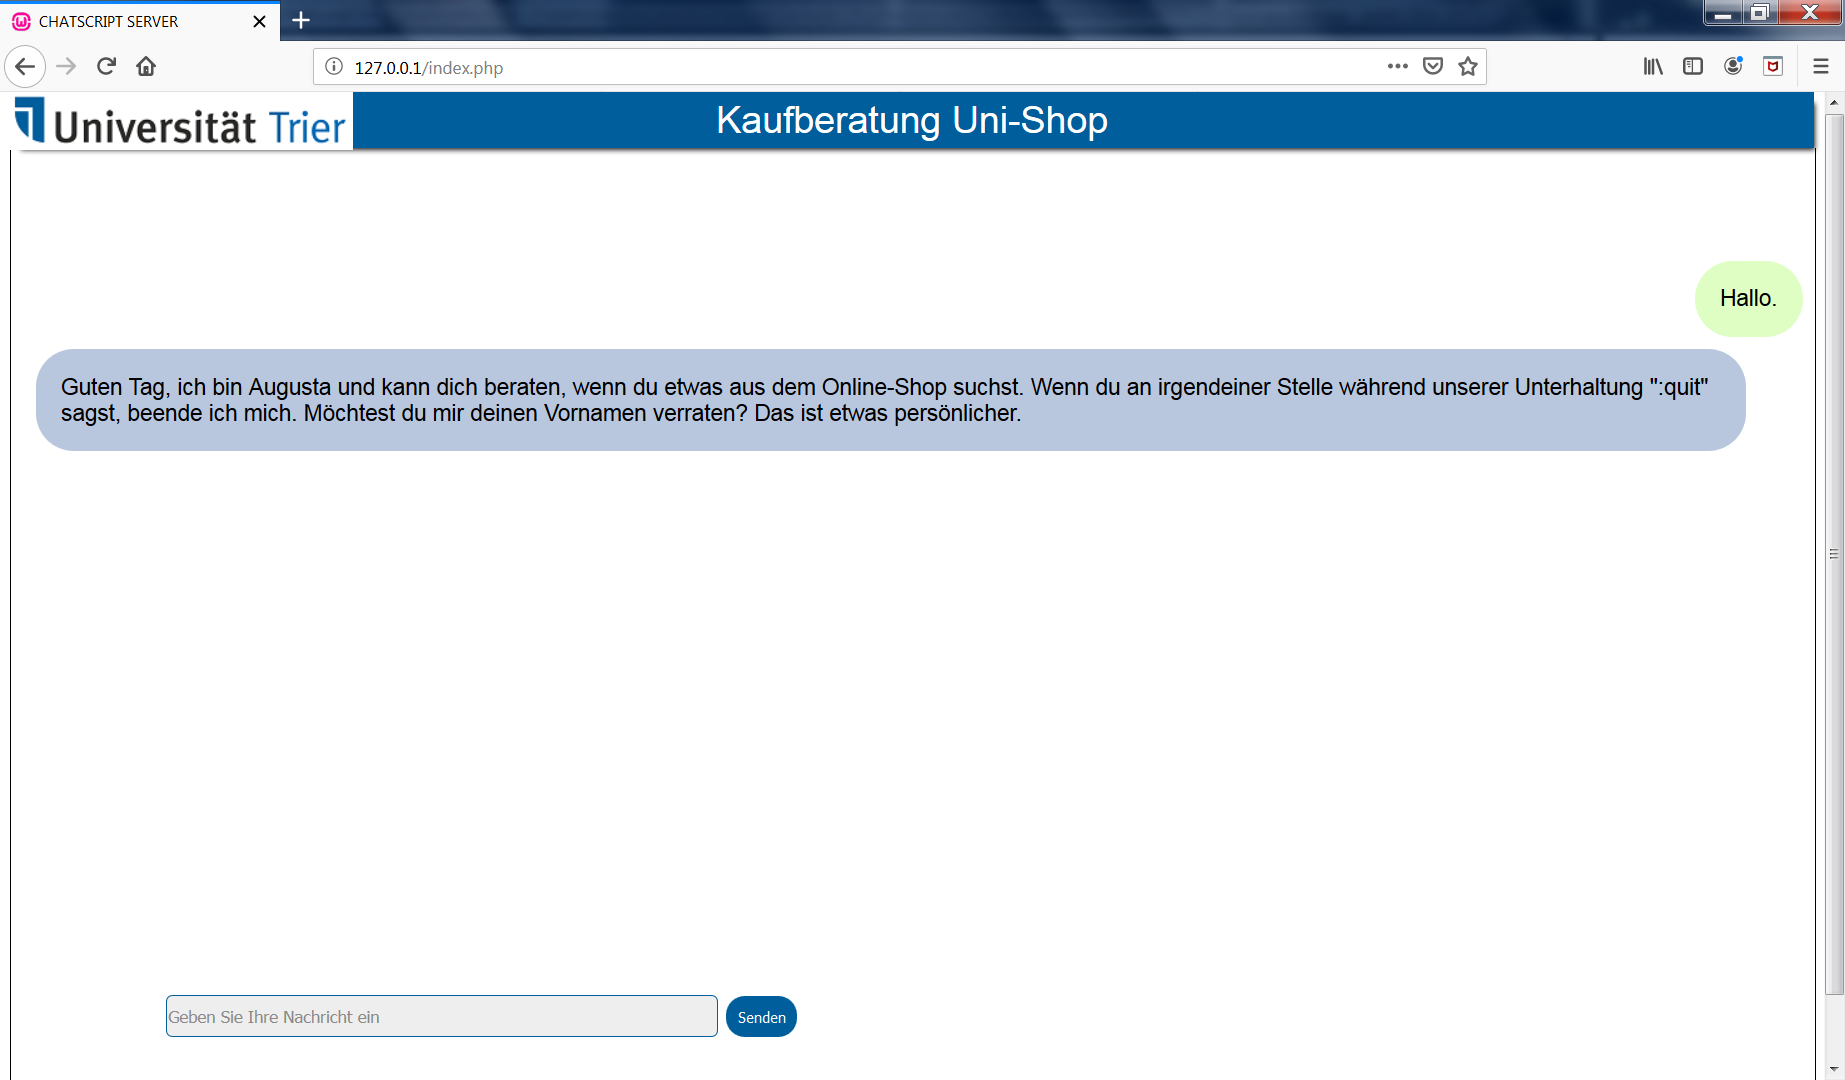
\includegraphics[width=8cm]{BILDER/gui.png}}
\end{center}
	\caption{Screenshot der Benutzerschnittstelle}
	\label{ScreenshotGUI}
\end{figure}

\chapter{Probleme}
\label{sec:Probleme}

Dieses Kapitel behandelt Schwierigkeiten, die bei der Arbeit mit ChatScript aufgetaucht sind und haben für uns ein ernstes und großes Hindernis dargestellt. Im Falle des zweiten Problems haben wir auch keine Lösung gefunden.\\


\section{Zwei-Query-Problem}
\label{Section: Zwei-Query Problem}

Ein Problem, für das ein Workaround gefunden werden konnte, war das 'Zwei-Query-Problem'. Dieses Problem ist in den allen Versionen vorhanden und tritt wegen einem der folgenden Fehler auf:

\begin{enumerate}
\item {Suche auf einer vor der Nutzung existierenden Datenbank}
\item {Fehlschlag in Queries}
\end{enumerate}  

Ersteres tritt auf, wenn man mit Hilfe des Befehls \lstinline|:build onesentence| oder Ähnliches den Bot, hier onesentence, neu kompiliert. Dies hat den Ursprung darin, dass der Bezeichner für die Datenbanken per Client mit einer Zufallszahl konkateniert wird und jeder \lstinline|:build|-Befehl dieselbe Zufallszahl generiert. Wird eine Tabelle nach ihrer Nutzung nicht gelöscht, dann tritt dieser Fehlschlag auf.\\
Dieses Problem erscheint in dieser Form nicht außerhalb des Testens, da es unwahrscheinlich ist, dass zwei Tabellen mit demselben Bezeichner zufallsgeneriert werden. Die Komplikation entsteht nicht, wenn ein Bot regelmäßig, das heißt durch Verabschiedung in Ende, beendet wird. Man kann dieses Problem manuell durch explizite \lstinline|drop|-Befehle außerhalb von Chatscript behandeln.\\
Zweiteres tratt auf, wenn mit den angegebenen Eigenschaften kein Produkt gefunden werden konnte. Wenn kein Produkt gefunden werden kann, ist dem Skript zu Folge in den Zustand \texttildelow ende.SETNULLANDREP überzugehen, um eine neue Suche zu gewährleisten. Nach der Programmlogik müssten hier die einzelnen Regeln bis zu der Datenbanksuche wieder iteriert werden, um Nutzerangaben zu sammeln. Stattdessen versuchte der Bot nach dem Zurücksetzen der Variablen, erneut eine Suche mit NULL-Variablen auszuführen, indem er eigenständig in SUMMARY sprang und ohne eine Antwort abzuwarten eine Suche startete.\\
Dieses Problem wurde größtenteils umgangen, indem man den Nutzer mehrmals hintereinander fragt, ob man eine neue Suche ausführen will. Der Ursprung dieses Problems bleibt jedoch ungeklärt. Eine Vermutung ist, dass ChatScript intern Regeln, die bereits besucht worden sind, markiert, um nicht erneut von alleine in jene Regeln überzugehen und so Wiederholungen im Gesprächsablauf zu vermeiden \citep{chatscript2019}.\\


\section{Probleme mit der GUI}
\label{sec: Probleme mit der GUI}

Bei dem Testen der GUI fallen einige Probleme auf: 

\begin{enumerate}
\item{Fehlender Support von PostgreSQL-Server für Mac und Linux}
\item{Server mit PostgreSQL-Unterstüzung vs. Server ohne PostgreSQL-Unterstüzung}
\end{enumerate}

Das Testen der GUI erfolgte durch das Hosten auf Localhost (127.0.0.1) der durch ChatScript bereitgestellten Dateien im Ordner \textit{SERVER BATCH FILES} \citep{chatscript2019}. Während das Aufsetzen eines Servers auf Windows recht einfach war, fiel schnell auf, dass einige unvorhergesehene Probleme auftraten. 

\subsection{Fehlender Support von PostgreSQL-Server für Mac und Linux}
\label{sec:Fehlender Support von PostgreSQL-Server für Mac und Linux}

In der Dokumentation für ChatScript wird beschrieben, wie ein Server ohne Postgres-Unterstützung auf Windows, Mac und Linux-Distributionen aufzusetzen ist. Für Windows wird die .bat-Datei \textit{LocalPgServer.bat} mitgeliefert, sodass das Aufsetzen eines Servers auf Windows keine Probleme bereitet. Im Gegensatz dazu wird nichts über Server mit Postgres-Support für Linux oder Mac in der Dokumentation erwähnt. Nach mehreren erfolglosen Versuchen wurde im Forum für Chatbots \cite{cb5} nachgefragt, wobei diese Frage unbeantwortet blieb. 

\subsection{Server mit PostgreSQL-Unterstüzung vs. Server ohne PostgreSQL-Unterstüzung}
\label{sec: Server mit PostgreSQL-Unterstüzung vs. Server ohne PostgreSQL-Unterstüzung}

Ein weiteres Problem bei dem Testen der GUI war, dass der Bot verschiedene Verhaltensweisen je nach .bat-Datei aufweist. So entspricht der Programmablauf des Bots dem der Konsolenausgabe, wenn ein Server ohne Postgres-Support, zum Beispiel durch \textit{LocalServer.bat}, eingerichtet wird. Hier verhält sich der Bot in den Zustandsübergängen identisch zu der Konsolenausgabe, mit dem Unterschied, dass der Nutzer  bei der GUI / des Webinterfaces die erste Eingabe machen muss.\\
Das bedeutet, dass bis zum Zeitpunkt der Datenbankabfrage in Dbsearch keine Probleme auftreten. Zu Schwierigkeiten kommt es in diesem Fall verständlicherweise erst dann, wenn eine Datenbankabfrage ausgeführt werden muss, da hier keine Unterstützung für PostgreSQL besteht.\\
Im Gegensatz dazu gab es in vielerlei Hinsicht Probleme mit der Einrichtung eines Servers mit Postgres-Unterstüzung. Bei einigen Anläufen startete der Bot gar nicht, im besten Fall wird \texttildelow dbsearch.RESPONSE erreicht, jedoch geht der Bot von dort aus in keine weitere Regel, sondern iteriert weitergehend auf \texttildelow dbsearch.RESPONSE.\\
In vielen Versuchen erwiesen sich Übergänge in Regeln mit \lstinline|^reuse ()| als problematisch. Bei Aufsetzen des Servers mit \textit{LocalPgServer.bat}, ist es vorgekommen, dass einige der vorgesehenen Regelübergänge per \lstinline|^reuse()| nicht aktiviert wurden. \\
Da Probleme mit \textit{LocalPgServer.bat} nicht in der Dokumentation von ChatScript behandelt werden und der Macher und Entwickler von ChatScript, Bruce Wilcox, nicht auf Nachfragen mit dem Hosten eines Servers mit Postgres-Unterstützung antwortet \cite{cb5}, konnten alle Probleme mit dem Server mit Postgres-Unterstützung zeitnah nicht gelöst werden.\\
Es besteht unsererseits die Vermutung, dass es bei \textit{LocalPgServer.bat} Schwierigkeiten mit der User-Datenbank gibt, die ChatScript automatisch erstellt. In der Datenbank \textit{user} werden die einzelnen User mit Name und deren Protokolle abgespeichert. Diese Protokolle sind auch über den Ordner \textit{USER} zugänglich und tragen den Namen \textit{topic\_username\_botname.txt}. Interessanterweise wird bei \textit{LocalPgServer.bat} zwar ein Protokoll für den Benutzer angelegt, das existiert aber nur in der Datenbank und erscheint in dem USERS-Ordner nicht. Zudem bricht es nach SUMMARY ab, als wäre der Bot noch immer in diesem Zustand, obwohl die Datenbanksuche schon ausgeführt wurde und er aufgrund des ausgegebenen Textes schon in der Regel RESPONSE sein müsste.\\
Wie bereits erwähnt, tritt dieses Problem bei der Version über die Konsole und \textit{LocalSever.bat} nicht auf. Hier die Protokollführung nicht ab und die entsprechenden Protokolle sind über USERS einsehbar.\\
In der Datei \textit{bugs.txt} aus dem Ordner \textit{LOGS} wird das Problem folgendermaßen beschrieben: \lstinline{Postgres filessys write failed for USERS/topic\_127001\_augusta.txt}. Eine Suche über Google ergab, dass diese Beschreibung schon bei Schwierigkeiten mit ChatScript und dem Amazon Server aufgetaucht war (\url{https://www.chatbots.org/ai_zone/viewthread/3664/}). Die dortige Lösung das Problems, das Unique-Constraint der Relation \textit{userfiles} zu entfernen, haben wir auf unseren Fall übertragen und ausprobiert, allerdings hat dies nicht den gewünschten Effekt gehabt.\\
Aufgrund Zeitmangels, mangelnder Dokumentation und fehlender Einsicht in die Binärdateien bzw. Konfiguration ist dieses Problem bis dato nicht gelöst. Die genaue Fehlerquelle konnte nicht ausfindig gemacht werden und es ist ein Rätsel, warum auch Nicht-Postgres-Abläufe sich bei dem Server mit Postgres-Unterstützung anders verhalten als ohne Postgres-Unterstützung.

%\chapter{Fazit}
\label{sec:Fazit}



\backmatter					% Anhang

\chapter{Beispiele zum Dialogablauf}
\label{sec:Beispieldialog}

Im Folgenden gibt es einige Beispiele für den Ablauf des Dialogs zwischen Chabot und Kunde, die wir vor und teilweise auch während des Programmieren geschrieben haben. So enthält beispielsweise Dialog 3 gegenüber Dialog 1 bereits Änderungen, die wir mit in das Programm übernommen haben.\\
Die kursiv geschriebenen Ausgaben des Chatbots (z. B. \textit{ABC} oder \textit{Beschreibung}) werden in der Realität durch Name, Beschreibung und Ähnliches ersetzt.\\

\Large\textbf{Dialog 1: Abgelehntes Produkt}\\
\normalsize
Dieser Dialog war der erste, der für den Chatbot geschrieben wurde. Er stellt eine Situation dar, in der ein Kunde das ihm vorgeschlagene Produkt ablehnt, wonach der Chatbot erneut suchen muss.\\
In der ersten Vorstellung hatten wir noch geplant, dass der Kunde bei Interesse nach Produktinformationen fragen kann. Im Verlauf des Projekts haben wir uns gegen das Nachfragen entschieden und präsentieren dem Kunden den Namen, die Beschreibung und den Preis sofort (s. \ref{sec:AusgabeWarenkorb}). Zum einen ist diese Variante einfacher und zum anderen sind Beschreibung und Name zusammen aussagekräftiger als der Name alleine.
Außerdem fiel beim Schreiben des Dialogs auf, dass Fragen mit oder zu vermeiden sind, da manche Personen dazu neigen, solche Fragen mit "`Ja."' und "`Nein."' zu beantworten.
\begin{center}
\begin{tabular}{p{2,5cm}p{12,6cm}}
	\textsc{Chatbot:} & Hallo. Suchen Sie ein Geschenk oder ein Produkt für einen bestimmten Zweck? \\
	\textsc{Kunde:} & Ich suche ein Geschenk.\\
	\textsc{Chatbot:} & Nach was für einer Art (von Geschenk) suchen Sie? Ich kann Ihnen folgende Optionen anbieten: Geschenk, Gastgeschenk, Mitbringsel, Erinnerungsstück.\\
	\textsc{Kunde:} & Gastgeschenk. \\
	\textsc{Chatbot:} & Ich kann Ihnen dieses Produkt empfehlen: \textit{ABC}. Möchten Sie weitere Informationen darüber oder soll ich weitersuchen?\\
	\textsc{Kunde:} & Weitere Informationen. \\
	\textsc{Chatbot:} & \textit{Beschreibung}. Ist es das, was Sie gesucht haben?\\
	\textsc{Kunde:} & Nein. \\
	\textsc{Chatbot:} & Ich werde weitersuchen. Das kann ich noch empfehlen: \textit{DEF}. Möchten Sie weitere Informationen darüber oder soll ich weitersuchen? \\
	\textsc{Kunde:} & Ich will mehr Infos. \\
	\textsc{Chatbot:} & \textit{Beschreibung.} War es das, was Sie gesucht haben? \\
	\textsc{Kunde:} & Wie viel kostet das? \\
	\textsc{Chatbot:} & \textit{DEF} kostet \textit{9,50} Euro. Möchten Sie \textit{DEF} erwerben?\\
	\textsc{Kunde:} &  Ja.\\
	\textsc{Chatbot:} & Sie können das Ticket für \textit{DEF} über den Tukan erwerben und dieses dann in der Pressestelle oder im Shop abgeben. Suchen Sie ein weiteres Produkt? Ein Geschenk oder einen Artikel für einen bestimmten Zweck?\\
	\textsc{Kunde:} & Nein. Tschüss. \\
	\textsc{Chatbot:} & Auf Wiedersehen.\\
	\end{tabular}
\end{center}
\vspace{12pt}


\Large\textbf{Dialog 2: Zweite Suche}\\
\normalsize
In diesem Dialog wird nach einem ersten Treffer noch nach einem zweiten Produkt mit verschiedenen Kriterien gesucht. Nach der Bestätigung, dass nach einem neuen Produkt gesucht werden soll, beginnt der Dialog ab der Frage nach einem Geschenk oder Anwendungszweck von vorne.\\
Da wir die Kategorien der Geschenkideen und Anwendungsgebiete automatisch ausgeben wollten, hat sich hier die Ausgabe ein wenig verändert. Die Oder-Frage des vergangenen Dialogs haben wir herausgenommen. Dazu wird die Information über der Uni-Shop erst dann ausgegeben, wenn der Kunde nicht mehr möchte, damit auch bei mehreren Suchen dieser Satz nur einmal erwähnt wird.
\vspace{8pt}
\begin{center}
\begin{tabular}{p{2,5cm}p{12,6cm}}
	\textsc{Chatbot:} & Hallo. Suchen Sie ein Geschenk oder ein Produkt für einen bestimmten Zweck? \\
	\textsc{Kunde:} & Ich suche ein Geschenk.\\
	\textsc{Chatbot:} & Nach was für einer Art Geschenk suchen Sie? Ich kann Ihnen folgende Optionen anbieten: Geschenk. Gastgeschenk. Mitbringsel. Erinnerungsstück.\\
	\textsc{Kunde:} & Ich will ein Gastgeschenk. \\
	\textsc{Chatbot:} & Ich kann Ihnen dieses Produkt empfehlen: \textit{ABC}. Möchten Sie weitere Informationen dazu? Wenn Sie möchten, kann ich weitersuchen. \\
	\textsc{Kunde:} & Informationen. \\
	\textsc{Chatbot:} & \textit{Beschreibung}. Ist es das, was Sie gesucht haben?\\
	\textsc{Kunde:} & Ja. \\
	\textsc{Chatbot:} & Möchten Sie ein weiteres Produkt suchen? \\
	\textsc{Kunde:} & Ja. \\
	\textsc{Chatbot:} & \textit{Beschreibung.} Suchen Sie ein Geschenk oder ein Produkt für einen bestimmten Zweck?\\
	\textsc{Kunde:} & Bestimmter Zweck. \\
	\textsc{Chatbot:} & Wofür benötigen Sie das Produkt: Ich kann Ihnen folgende Kategorien anbieten: Accessoire. Alltag. EssenTrinken. Deko. Uni. \\
	\textsc{Kunde:} &  Alltag.\\
	\textsc{Chatbot:} & Ich kann Ihnen dieses Produkt empfehlen: \textit{DEF}. Möchten Sie weitere Informationen dazu? Wenn Sie möchten, kann ich weitersuchen. \\
	\textsc{Kunde:} & Wie teuer ist das? \\
	\textsc{Chatbot:} & \textit{DEF} kostet \textit{9,50} Euro. War es das, was Sie gesucht haben? \\
	\textsc{Kunde:} & Ja. \\
	\textsc{Chatbot:} & Möchten Sie ein weiteres Produkt suchen? \\
	\textsc{Kunde:} & Nein. Tschüss. \\
	\textsc{Chatbot:} & Sie können das Ticket für die Produkte über den Tukan erwerben und dieses dann in der Pressestelle oder im Shop abgeben. Auf Wiedersehen.\\
	\end{tabular}
\end{center}
\vspace{12pt}


\Large\textbf{Dialog 3: Suche mit genaueren Kriterien und Warenkorb}\\
\normalsize
Dieser Dialog ist etwas später entstanden. Hier gibt es bereits die Möglichkeit, zusätzlich zu Geschenk und Anwendung noch weitere Kriterien wie die Ausführung oder den Preis anzugeben. In den Onesentence-Chatbots ist dies in der Variante implementiert, wie im Dialog beschrieben: Der Kunde gibt die Kriterien in einem Satz an und der Chatbot weist Variablen zu. In KeyExProdukteigenschaften wird einzeln nach Name, Art, Ausführung und Preis gefragt. Dies hatten wir zu Beginn geschrieben, um zumindest einen Dialog führen und die Variablen zuzuweisen zu können und dann es später die schwierigere Variante mit einem einzigen Satz auszutauschen. Allerdings stellte sich im Anwendungstest (s. Ergebnis des Usability Testing) heraus, dass vom Benutzer der Dialog mit den einzelnen Abfragen als einfacher empfunden wird.\\
Dazu wird beim Produktvorschlag gleich die Beschreibung mit ausgegeben und der Kunde erhält die Möglichkeit, sich anzusehen, was er bereits ausgewählt hat.\\
Zudem duzt der Chatbot den Kunden und fragt nach einem Namen, um persönlicher sein zu können.
\vspace{8pt}
\begin{center}
\begin{tabular}{p{2,5cm}p{12,6cm}}
	\textsc{Chatbot:} & Hallo. Möchtest du mir deinen Namen verraten? Das ist etwas persönlicher. \\
	\textsc{Kunde:} & XYZ.\\
	\textsc{Chatbot:} & Hallo, \textit{XYZ}. Du bist hier, um etwas zu kaufen, oder? \\
	\textsc{XYZ:} & Ja. \\
	\textsc{Chatbot:} & Dann fangen wir an. Suchst du ein Geschenk oder ein Produkt für einen bestimmten Zweck? \\
	\textsc{XYZ:} & Geschenk.\\
	\textsc{Chatbot:} & Nach was für einer Art Geschenk suchst du? Ich kann dir folgende Optionen anbieten: Geschenk, also zum Beispiel zum Geburtstag oder zu Weihnachten. Gastgeschenk. Mitbringsel. Erinnerungsstück.\\
	\textsc{XYZ:} & Ein Gastgeschenk. \\
	\textsc{Chatbot:} & Hier kannst du in einem Satz noch weitere Kriterien für das gesuchte Produkt hinzufügen. Den Namen oder die Art des Produkts, zum Beispiel. Zudem bieten wir manche Produkte in verschiedenen Farben oder Sprachen an. Außerdem kannst du eine preisliche Obergrenze festlegen.\\
	\textsc{XYZ:} & Ein Buch in Englisch für 10 Euro.\\
	\textsc{Chatbot:} & Ich wiederhole: Du möchtest ein Gastgeschenk. Es handelt sich dabei um ein Buch. Es ist in Englisch und kostet maximal 10 Euro. Stimmt das so? \\
	\textsc{XYZ:} & Ja. \\
	\textsc{Chatbot:} & Ich kann dir dieses Produkt empfehlen: \textit{ABC}. \textit{Beschreibung.} Ist es das, was du gesucht hast? Wenn du möchtest, kann ich weitersuchen. \\
	\textsc{XYZ:} & Ja. \\
	\textsc{Chatbot:} & Möchtest du ein weiteres Produkt suchen? Du kannst dir auch ansehen, was du bereits ausgewählt hast. \\
	\textsc{XYZ:} & Ich will mir ansehen, was ich bereits ausgewählt habe. \\
	\textsc{Chatbot:} & Du hast \textit{1} Produkt ausgewählt. Es ist \textit{ABC}. Die Beschreibung lautet \textit{Beschreibung.} Es kostet \textit{6,50} Euro. Möchtest du ein weiteres Produkt suchen? \\
	\textsc{XYZ:} & Nein.\\
	\textsc{Chatbot:} & Du kannst das Ticket für die Produkte über den Tukan erwerben und dieses dann in der Pressestelle oder im Shop abgeben. Auf Wiedersehen.\\
	\end{tabular}
\end{center}
\vspace{12pt}


\Large\textbf{Dialog 4: Kein Ergebnis / Fehler bei der Suche}\\
\normalsize
Dieser Dialog stellt die Möglichkeit, dass es bei der Suche zu einem Fehler kommt. Wenn der Chatbot kein Produkt findet, wird es statt "`Oh, tut mir leid, da habe ich mich verrechnet. Lass uns von vorne anfangen."' "`Ich habe leider kein Produkt gefunden, das auf deine Kriterien passt. Versuchen wir es nochmal mit anderen Kriterien"' ausgeben.\\
Dazu kann der Kunde hier den Bot auch mitten im Dialog beenden, was im Chatbot OnesentenceGoodbye implementiert ist.
\vspace{8pt}
\begin{center}
\begin{tabular}{p{2,5cm}p{12,6cm}}
	\textsc{Chatbot:} & Hallo. Du kannst jederzeit "`Tschüss"' sagen, wenn du mich beenden  Möchtest du mir deinen Namen verraten? Das ist etwas persönlicher. \\
	\textsc{Kunde:} & Nein.\\
	\textsc{Chatbot:} & Das kann ich verstehen. Du bist hier, um etwas zu kaufen, oder? \\
	\textsc{Kunde:} & Ja. \\
	\textsc{Chatbot:} & Dann fangen wir an. Suchst du ein Geschenk oder ein Produkt für einen bestimmten Zweck? \\
	\textsc{Kunde:} & Geschenk.\\
	\textsc{Chatbot:} & Nach was für einer Art Geschenk suchst du? Ich kann dir folgende Optionen anbieten: Geschenk, also zum Beispiel zum Geburtstag oder zu Weihnachten. Gastgeschenk. Mitbringsel. Erinnerungsstück.\\
	\textsc{Kunde:} & Gastgeschenk. \\
	\textsc{Chatbot:} & Hier kannst du in einem Satz noch weitere Kriterien für das gesuchte Produkt hinzufügen. Den Namen oder die Art des Produkts, zum Beispiel. Zudem bieten wir manche Produkte in verschiedenen Farben oder Sprachen an. Außerdem kannst du eine preisliche Obergrenze festlegen.\\
	\textsc{Kunde:} & Englisch Buch 10.\\
	\textsc{Chatbot:} & Ich wiederhole: Du möchtest ein Gastgeschenk. Es handelt sich dabei um ein Buch. Es ist in Englisch und kostet maximal 10 Euro. Stimmt das so? \\
	\textsc{Kunde:} & Ja. \\
	\textsc{Chatbot:} & Oh, tut mir leid, da habe ich mich verrechnet. Lass uns von vorne anfangen. Suchst du ein Geschenk oder ein Produkt für einen bestimmten Zweck? \\
	\textsc{Kunde:} & Tschüss. \\
	\textsc{Chatbot:} & Du kannst das Ticket für die Produkte über den Tukan erwerben und dieses dann in der Pressestelle oder im Shop abgeben. Auf Wiedersehen.\\
	\end{tabular}
\end{center}


%\textsc{Chatbot:} & \\
%\textsc{XYZ:} & \\

\chapter{Ergebnis des Usability Testing}
\label{sec:UsabilityTesting}

Anfang Juni haben wir unser Programm einer kleiner Evaluierung unterzogen. Die Testgruppe bestand aus zwei Personen, die ein paar Mal mit Augusta gesprochen haben. Im Folgenden findet sich die Zusammenfassung dieses kleinen Usability Testings.\\
Ein Problem dabei war allerdings, dass das Programm zu diesem Zeitpunkt noch einige Bugs aufwies und nicht voll funktionsfähig war. Doch ein kurzes Feedback war möglich. Getestet wurde zudem nur eine Version auf der Konsole.
\vspace{10pt}


Zu Beginn gibt zwei mal in anderer Formulierung die Frage, ob der Kunde hier sei, um etwas zu kaufen (aus INTRO). Diese Fragen, vor allem in doppelter Ausführung, wurden nicht nur als unnötig sondern auch als nervig empfunden. Ebenso wird die Frage angezeigt, wenn der Kunde nach einem Fehler bei der Suche neu anfangen muss. Auch dies war für die Benutzer störend. \\
Verwirrend erschien des Weiteren die Angabe der Kategorien aus Geschenkidee (FIRSTQ). So sei bei "`Geschenk, also zum Beispiel zum Geburtstag oder zu Weihnachten. Gastgeschenk. Mitbringsel. Erinnerungsstück."' nicht klar, dass "`Geschenk"', "`Gastgeschenk"', "`Mitbringsel"' und "`Erinnerungsstück"' um die Auswahlmöglichkeiten handle und es wurde angenommen, dass man auch "`zum Geburtstag"' oder "`zu Weihnachten"' eingeben könne. Generell führte die Ambiguität des Begriffs "`Geschenk"' verwirrend zu Unklarheit.\\
Kritisch betrachtet wurde auch, dass Augusta "`Gerne."' als Ersatz für "`Ja."' nicht akzeptiere.\\
Außerdem zeigten sich die Benutzer von den vielen Eingabemöglichkeiten in KeyExOnesentence beim Erfragen von zusätzlichen Produktkriterien überfordert. So wusste beispielsweise eine Testperson nicht reicht, "`wie genau man das eingeben soll."' So sei unklar gewesen, ob man nur die Begriffe oder einem vollständigen Satz eingeben solle. Ein zweiter Test mit KeyExProdukteigenschaften ist als einfacher empfunden worden, da hier der Bot den Benutzer mit gezielten Fragen nach Produktname, Ausführung und Preis führe.
\vspace{10pt}


Als Reaktion auf die Tests haben wir die doppelte Frage nach der Kaufabsicht aus INTRO herausgenommen. Inzwischen geht Augusta von Anfang an davon aus, dass der Kunde etwas kaufen möchte oder zumindest nach etwas sucht.\\
Die Ausgabe der Kategorien haben wir vor Ort noch in "`Geschenk, Gastgeschenk, Erinnerungsstück und Mitbringsel"' umformuliert. Zudem fragt der Chatbot am Anfang von FIRSTQ ob der Kunde "`etwas zum Verschenken oder für einen besonderen Zweck"' suche, wodurch der Begriff "`Geschenk"' desambiguiert werden soll. Die Testpersonen reagierten auf diese beiden Änderungen sehr positiv. Es sei nun verständlicher. \\
Ursprünglich war KeyExProdukteigenschaften nur als Übergangslösung bis zur Fertigstellung von KeyExOnesentence gedacht. Allerdings haben wir uns dazu entschieden, aufgrund der Bemerkungen der Testpersonen, einen zweiten Chatbot mit KeyExProdukteigenschaften anstatt KeyExOnesentence als Alternative zur Verfügung zu stellen.




%Glossar ausgeben
%\printglossary[style=altlist,title=Glossar]
\printglossary

\listoftables				% Tabellenverzeichnis
\listoffigures			% Abbildungsverzeichnis

\newpage

%\setbibpreamble{Präambel}		% Text vor dem Verzeichnis
%\bibliographystyle{dinat}
%\bibliography{bibliographie}	% Sie benötigen einen *.bib-Datei

%%%%%%%%%%%%%%%%%%%%%%%%%%%%%%%%%%%%%%%%%%%%%%%%
% B I B L I O G R A P H I E
%%%%%%%%%%%%%%%%%%%%%%%%%%%%%%%%%%%%%%%%%%%%%%%%

\renewcommand{\baselinestretch}{1}\normalsize 	%Zeilenabstand innerhalb der Angaben
\cleardoublepage
\addcontentsline{toc}{chapter}{\bibname}	%Bib. im Inhaltsvz.

\bibliography{CL-bib}					%Bibliographiedatenbank
\bibliographystyle{CL-DE}		%Zitierstruktur - natbib muss deklariert sein!

\nocite{*} 		%optional - gibt die gesammte Bib-Datenbank aus ansonsten werden nur 
%die zitierten Werke ausgegeben

%%%%%%%%%%%%%%%%%%%%%%%%%%%%%%%%%%%%%%%%%%%%%%%%
\end{document}
